% !TEX program=xelatex
%\documentclass[notes=show]{beamer}
\documentclass[notes=onlyslideswithnotes,notes=hide]{beamer}
%\documentclass[notes=hide]{beamer}
%\documentclass[notes=only]{beamer}
%\documentclass[10pt,letterpaper]{article}
%\usepackage{beamerarticle}

%\documentclass{beamer}
%\usepackage{pgfpages}
%\setbeameroption{show notes on second screen}

\usepackage{genchem}
\usepackage{lecture}
\usepackage{multicol}
%\usepackage{modiagram}
\usepackage{elements}
%\usepackage{ccicons}

\renewcommand*\printangularmomentum[1]{#1}

\usepackage{orbitalfilling}[2019/02/14]

\title{The Elements and the Periodic Table}
\subtitle{Chapter 3}
\institute[CHEM115 Bloomsburg University]{CHEM115 --- Chemistry for the Sciences I \\ Bloomsburg University}
\author{D.A. McCurry}
\date{Fall 2020}

\begin{document}

\maketitle
\mode<article>{\thispagestyle{fancy}}

%\mode<presentation>{\input{"../../Exams/Exam 1/Results/Exam1Summary"}}

\frame{\section{Organizing and Classifying Elements}
	\begin{learningobjectives}
		\item Explain how the periodic table is organized.
		\item Connect the concept of quantum numbers with electron
			location in an atomic orbital.
		\item Fill electron orbitals appropriately using the Pauli
			Exclusion Principle.
	\end{learningobjectives}
}

\begin{frame}{Elemental Patterns}
	\begin{itemize}
		\item<1-> We are familiar with numerous \emph{physical}
			and \emph{chemical} properties.%
			\begin{multicols}{2}%
				\begin{itemize}%
					\item Boiling point
					\item Solubility
					\item Color
					\item State
				\end{itemize}
			\end{multicols}

		\item<2-> How do we go from $H\Psi = E\Psi$
			%\begin{tikzpicture}[baseline=(current bounding
			%	box.west),scale=0.6]
			%	\begin{axis}[axis x line=none,
			%		axis y line=none,
			%		domain=0:4,
			%		height=1in,
			%		width=2in,ymax=1,ymin=-0.3]
			%		\addplot[primary,thick,samples=200]
			%		{0.25*sin(x*180)};
			%		\node[anchor=north] at (current bounding
			%		box.north) {$H\Psi = E\Psi$};
			%	\end{axis}
			%\end{tikzpicture}
			to the \emph{properties} we observe in the \emph{macro}
			world?
		\item<3-> More importantly, is there an \alert{easy} way to
			predict properties of elements?
	\end{itemize}
\end{frame}

\begin{frame}{Dmitri Mendeleev (1869)}
	\only<1>{%
		\begin{center}
			\includegraphics[scale=0.3]{density.jpg}
		\end{center}
	
		\begin{block}{The Periodic Law}
			When the elements are arranged in order of increasing mass,
			certain sets of properties recur periodically.
		\end{block}
	}
	\only<2>{%
		Elements could be \alert{grouped} into columns based on their properties.

		\begin{center}
			\begin{tikzpicture}
				\node(ptable)
				{\includegraphics[width=0.9\linewidth]{mendeleev-ptable.png}};
				\node[anchor=south east] at (ptable.south east)
				{\includegraphics[scale=0.4]{mendeleev-wiki.jpg}};
			\end{tikzpicture}
		\end{center}
	}
	\only<3>{%
		Using Mendeleev's early periodic table, he could even predict properties
		for elements that had yet to be discovered:

		\bigskip

		\includegraphics[width=\linewidth]{gallium-germanium.jpg}
	}
\end{frame}

\begin{frame}{The Modern Periodic Table}
	\centering

	\includegraphics[width=\linewidth]{modern-ptable.jpg}
\end{frame}

\begin{frame}{What determines these trends?}
	\begin{itemize}
		\item Recall: chemistry is the study of the \alert{structure} of
			the particles that compose matter.
		\item The interactions of electrons determine the overall
			structure of molecules.
		\item We therefore need to understand \alert{electron
			configurations} --- the locations of electrons within an
			atom.
	\end{itemize}

	\pause%

	\begin{example}
	What is the electron configuration of hydrogen in the ground
	state?
	\end{example}

	\note<2->{%
		\begin{itemize}
			\item How many electrons does hydrogen have?
			\item Where might this electron exist in the ground
				state?
				\begin{itemize}
					\item Principal quantum number ($n = 1$)
					\item Angular momentum quantum number
						($l = 0$)
					\item Magnetic momentum quantum number
						($m_l = 0$)
				\end{itemize}
		\end{itemize}

		\begin{equation*}
			1s^1
		\end{equation*}}
\end{frame}

\begin{frame}{Orbital Filling Diagrams}
	\begin{itemize}[<+->]
		\item Another method for indicating electron location is via
			\alert{orbital diagrams}.

			\begin{center}
				\begin{tikzpicture}
					\node[font=\Huge](up)
					{$\upharpoonleft\mathrel{\hphantom{\downharpoonright}}$};
					\draw[thick] (up.west) -- (up.east);
					\node[right = of up,font=\Huge](down)
					{$\mathrel{\hphantom{\upharpoonleft}}\downharpoonright$};
					\draw[thick] (down.west) -- (down.east);
					\node[right = of down,font=\Huge](both)
					{$\upharpoonleft\downharpoonright$};
					\draw[thick] (both.west) -- (both.east);
					\node[below = 2pt of up](plus) {$+\frac{1}{2}$};
					\node[below = 2pt of down] {$-\frac{1}{2}$};
					\node[below = 2pt of both]
					{$+\frac{1}{2}$, $-\frac{1}{2}$};
					\node[left = 10pt of plus]
					{$m_s\hspace{10pt}=$};
				\end{tikzpicture}
			\end{center}

		\item For hydrogen,

			\begin{center}
				\begin{tabular} {@{}*{3}{c}}
					\ch{H} & $1s^1$ & \electronup%
				\end{tabular}
			\end{center}

		\item What about multi-electron systems?
	\end{itemize}
\end{frame}

\begin{frame}{Adding an Electron: Helium}
	\begin{itemize}
		\item What is the electron configuration of \ch{He}?

			\pause%

			\begin{equation*}
				1s^2
			\end{equation*}

			\pause%

		\item What is the orbital diagram for Helium?

			\pause%

			\begin{center}
				\electron{$\upharpoonleft\upharpoonright$}?
				\qquad
				\pause%
				\electron{$\upharpoonleft\downharpoonright$}?
				\qquad
				\pause%
				\electron{$\downharpoonleft\downharpoonright$}?
			\end{center}
	\end{itemize}

	\pause%

	\begin{block}{Pauli Exclusion Principle}
		No two electrons in an atom can have the same four quantum
		numbers.
	\end{block}

	\pause%

	\begin{center}
		$1s^2 \rightarrow n = 1 \qquad l = 0 \qquad m_l = 0$

		so $m_s$ \alert{must} differ.

		\pause%

		\textbf{\usebeamercolor[fg]{alerted text}This also means we can only have 2 electrons per orbital!}
	\end{center}
\end{frame}

\begin{inclass}[c]
		\begin{tabularx}{\linewidth} {c >{\centering\arraybackslash}m{1in}
			>{\centering\arraybackslash}X}
		\toprule
		\bfseries Element & \bfseries \ch{e^{-}} Config & \bfseries Orbital
		Diagram \\ \midrule
		\parbox[c][4em][c]{0.5in}{\centering\ch{Li}} & \\
		\parbox[c][4em][c]{0.5in}{\centering\ch{Be}} & \\
		\parbox[c][4em][c]{0.5in}{\centering\ch{B} } & \\
		\bottomrule
	\end{tabularx}

	\note{%
		\begin{center}
		\begin{tabular} {*{3}{c}}
		\bfseries Element & \bfseries \ch{e^{-}} Config & \bfseries Orbital
		Diagram \\ 
		\parbox[c][4em][c]{0.5in}{\centering\ch{Li}} & $1s^22s^1$ & \electronboth\quad \electronup \\
		\parbox[c][4em][c]{0.5in}{\centering\ch{Be}} & $1s^22s^2$ & \electronboth\quad \electronboth\\
		\parbox[c][4em][c]{0.5in}{\centering\ch{B} } & $1s^22s^22p^1$ & \electronboth\quad
		\electronboth\quad \electronup\electronnone\electronnone \\
		\end{tabular}
\end{center}}
\end{inclass}

\begin{onyourown}%{0em}
	\begin{tabularx}{\linewidth} {c >{\centering\arraybackslash}m{1in}
			>{\centering\arraybackslash}X}
		\toprule
		\bfseries Element & \bfseries \ch{e^{-}} Config & \bfseries Orbital
		Diagram \\ \midrule
		\parbox[c][4em][c]{0.5in}{\centering\ch{Na}} & \\
		\parbox[c][4em][c]{0.5in}{\centering\ch{F} }& \\
		\parbox[c][4em][c]{0.5in}{\centering\ch{Cl}} & \\
		\bottomrule
	\end{tabularx}
\end{onyourown}

\vspace{\stretch{1}}

\frame{\section{Higher-Level Electron Configurations}
	\begin{learningobjectives}
	\item Explain why electrons fill orbitals in specific configurations.
	\item Understand how energy level differences play a role in electron
		configurations.
	\item Use the periodic table to fill electron orbitals.
	\end{learningobjectives}
}

\begin{frame}{Electrons are Repulsive}
	\begin{block}{Coulomb's Law}
		The potential energy ($E$) of two charged particles depends on
		their charges ($q_1$ and $q_2$) and on their separation ($r$):

		\begin{equation*}
			E = \frac{1}{4\pi e_0} \frac{q_1 q_2}{r}
		\end{equation*}
	\end{block}

	\begin{itemize}[<+->]
		\item More electrons means a larger negative charge density.
		\item \alert{Sublevel energy splitting} --- the electron-electron
			interactions cause the orbital energies of
			multi-electron systems to be different.
	\end{itemize}
\end{frame}

\begin{frame}{Single vs. Multi-Electron Orbital Energies}
	\begin{center}
		\includegraphics[scale=0.35]{degenerate-mcmurry.jpg}
	\end{center}

	For 1 electron systems, the sublevels are considered \alert{degenerate}
	--- they have the same energy.
\end{frame}

\begin{frame}{The Aufbau Principle}
	\begin{itemize}
		\item Energy levels typically follow the order:
			\begin{equation*}
				E~(s \text{~orbital}) < E~(p \text{~orbital}) <
				E~(d \text{~orbital}) < E~(f \text{~orbital})
			\end{equation*}
		\item We can therefore ``build up'' (\textit{aufbau} in German)
			the electron configurations of atoms from the lowest
			energy orbitals to the highest energy orbitals.
		\item For B, this is why the $s$ orbitals were completed before
			the $p$ orbitals:

			\begin{center}
				\begin{tabularx}{\linewidth} {c c X}
					\ch{B} & $1s^22s^22p^1$ &
					\electronboth\quad \electronboth\quad
					\electronup\electronnone\electronnone
				\end{tabularx}
			\end{center}
	\end{itemize}
\end{frame}

\begin{frame}{Hund's Rule}
	What about carbon?

	\begin{center}
		\begin{tabular} {*{3}{c}}
			\ch{C} & $1s^22s^22p^2$ & \electronboth\quad
			\electronboth\quad
			\electronboth\electronnone\electronnone \\
			& & \textit{or} \\
			& & \electronboth\quad \electronboth\quad
			\electronup\electronup\electronnone \\
		\end{tabular}
	\end{center}

	\pause

	When filling \alert{degenerate} orbitals, we \emph{must} fill them with
	parallel spins (all~$+\frac{1}{2}$ or all~$-\frac{1}{2}$) \alert{before}
	pairing the electrons.

	\pause

	\begin{itemize}
		\item It's all about \alert{lower energy}.
	\end{itemize}
\end{frame}

\begin{inclass}[c]
	\begin{tabularx}{\linewidth} {c
			>{\centering\arraybackslash}m{1in}
		>{\centering\arraybackslash}X}
		\toprule
		\bfseries Element & \bfseries \ch{e^{-}} Config & \bfseries Orbital
		Diagram \\ \midrule
		\parbox[c][4em][c]{0.5in}{\centering\ch{N}} & \\
		\parbox[c][4em][c]{0.5in}{\centering\ch{O}} & \\
		\parbox[c][4em][c]{0.5in}{\centering\ch{F} } & \\
		\parbox[c][4em][c]{0.5in}{\centering\ch{Ne} } & \\
		\bottomrule
	\end{tabularx}

	\note{
		\begin{tabular} {*{3}{c}}
			\toprule
		\bfseries Element & \bfseries \ch{e^{-}} Config & \bfseries Orbital
		Diagram \\ \midrule
		\ch{N} & $1s^22s^22p^3$ & \electronboth\quad
			\electronboth\quad
			\electronup\electronup\electronup \\
		\ch{O} & $1s^22s^22p^4$ & \electronboth\quad \electronboth\quad
			\electronboth\electronup\electronup\\
		\ch{F}  & $1s^22s^22p^5$ & \electronboth\quad
		\electronboth\quad \electronboth\electronboth\electronup \\
			\ch{Ne} & $2s^22s^22p^6$ & \electronboth\quad
		\electronboth\quad \electronboth\electronboth\electronboth \\
		\bottomrule

		\end{tabular}}
\end{inclass}

\vspace{\stretch{-1}}

\begin{onyourown}%{0em}
	\begin{tabularx}{\linewidth} {c
			>{\centering\arraybackslash}m{1in}
		>{\centering\arraybackslash}X}
		\toprule
		\bfseries Element & \bfseries \ch{e^{-}} Config & \bfseries Orbital
		Diagram \\ \midrule
		\parbox[c][4em][c]{0.5in}{\centering\ch{C} }& \\
		\parbox[c][4em][c]{0.5in}{\centering\ch{S} } & \\
		\parbox[c][4em][c]{0.5in}{\centering\ch{Mg}} & \\
		\bottomrule
	\end{tabularx}
\end{onyourown}

\vspace{\stretch{-1}}

\begin{frame}[t]{An Issue with Aufbau}
	\begin{itemize}[<+->]
		\item What is the electron configuration of vanadium (\ch{V})?
			\note<1>{
				\begin{enumerate}
					\item How many electrons does vanadium
						have?
						
						\alert{23}
					\item What order does the configuration
						fill in?
						
						\alert{\elconf{V}}
				\end{enumerate}
				}
			\item $3d$ orbitals are often \alert{higher} in energy
				than $4s$ orbitals, but \alert{lower} in energy
				than $4p$ orbitals.

				\only<2>{
					\medskip
				\begin{center}
					\includegraphics[scale=0.35, trim={0 0 0
					40pt}, clip]{energyordering.jpg}
				\end{center}}

			\item An easy-ish way of remembering how to fill
				orbitals:

				\note{
				\begin{center}
					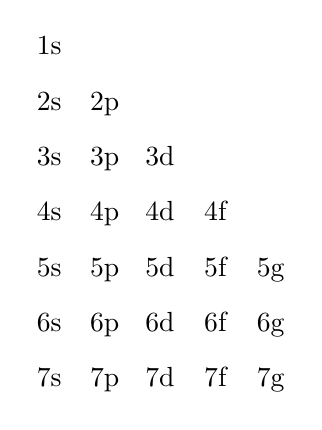
\begin{tikzpicture}[x=2em,y=2em,
						nodes={%
 						  execute at begin node=$,%
 						  execute at end node=$%
 						 },
						 every node/.style={anchor=base}]
						\tikzstyle{aufbau}=[thick,primary,->];
						\node(1s) at (0,0) {1s};
						\node(2s) at (0,-1) {2s};
						\node(2p) at (1,-1) {2p};
						\node(3s) at (0,-2) {3s};
						\node(3p) at (1,-2) {3p};
						\node(3d) at (2,-2) {3d};
						\node(4s) at (0,-3) {4s};
						\node(4p) at (1,-3) {4p};
						\node(4d) at (2,-3) {4d};
						\node(4f) at (3,-3) {4f};
						\node(5s) at (0,-4) {5s};
						\node(5p) at (1,-4) {5p};
						\node(5d) at (2,-4) {5d};
						\node(5f) at (3,-4) {5f};
						\node(5g) at (4,-4) {5g};
						\node(6s) at (0,-5) {6s};
						\node(6p) at (1,-5) {6p};
						\node(6d) at (2,-5) {6d};
						\node(6f) at (3,-5) {6f};
						\node(6g) at (4,-5) {6g};
						\node(7s) at (0,-6) {7s};
						\node(7p) at (1,-6) {7p};
						\node(7d) at (2,-6) {7d};
						\node(7f) at (3,-6) {7f};
						\node(7g) at (4,-6) {7g};
%						\mode<presentation>{
%						\visible<4->{\draw[aufbau]  (1s.north east) -- (1s.south west);}
%						\visible<5->{\draw[aufbau]  (2s.north east) -- (2s.south west);}
%						\visible<6->{\draw[aufbau]  (2p.north east) -- (3s.south west);}
%						\visible<7->{\draw[aufbau]  (3p.north east) -- (4s.south west);}
%						\visible<8->{\draw[aufbau]  (3d.north east) -- (5s.south west);}
%						\visible<9->{\draw[aufbau]  (4d.north east) -- (6s.south west);}
%						\visible<10->{\draw[aufbau] (4f.north east) -- (7s.south west);}
%						}
					\end{tikzpicture}
			\end{center}}
	\end{itemize}
\end{frame}

\begin{frame}{Electron Configurations from the Periodic Table}
	\centering
	\only<1>{\includegraphics[width=\linewidth,trim={0 0 0 30pt},clip]{orbitalblocks.jpg}}

	\only<2>{\includegraphics[width=\linewidth]{orbitalblocks-1.jpg}                     }

	\mode<article>{\clearpage}

	\only<3>{\includegraphics[width=\linewidth]{orbitalblocks-2.jpg}                     }
\end{frame}

\begin{frame}{Some Exceptions to Electron Configurations}
	\begin{itemize}
		\item The $4s$ and $3d$ orbitals are so close in energy that
			some elements do not follow the trends.
	\end{itemize}

	\begin{center}
		\includegraphics[scale=0.4]{transition-exceptions.jpg}
	\end{center}

	\begin{itemize}
		\item These exceptions are determined experimentally through
			spectroscopy (think atomic emission).
	\end{itemize}
\end{frame}

\begin{frame}{Shorthand Electron Configurations}
	As we build up the electron configuration for the larger atomic numbers,
	we can distinguish the \alert{inner} electron configurations from the
	\alert{outer} electron configurations:

	\begin{description}
		\item[Inner:] Completed suborbitals can be represented by a
			noble gas.
		\item[Outer:] Remaining electrons are indicated as before.
	\end{description}

	\textbf{Example:} For chlorine,
		\begin{equation*}
			\underbrace{\bm{1s^22s^22p^6}}_{\ch{[Ne]}}3s^23p^5
		\end{equation*}
		The abbreviated configuration for chlorine is therefore
		\begin{equation*}
			\ch{[Ne]}3s^23p^5
		\end{equation*}
\end{frame}

\begin{frame}{Core Shell vs. Valence Electrons}
	\only<1>{%
		Shorthand configurations are not just useful for simplicity!
		\begin{itemize}
			\item Noble gases are considered noble because they don't bond
				with other atoms.
			\item All electrons are paired and orbitals are in their most
				stable configuration.
			\item These inner electrons are considered \alert{core shell}
				electrons.
				\smallskip
				\begin{center}
			\includegraphics[scale=0.2]{coreshell-config.jpg}
		\end{center}
		\end{itemize}
	}

	\only<2>{%
		\begin{itemize}
			\item The outer, or \alert{valence}, electrons participate in
				reactions, bonding, etc.
			\item Note the arrangement of the periodic table places elements
				with the same number of valence electrons in the same
				\alert{groups}.
		\begin{center}
			\includegraphics[scale=0.4,trim={0 0 0 40pt},clip]{valence-electrons.jpg}
		\end{center}
			\item Atoms without a \alert{noble gas configuration} react to
				attain such a configuration.
		\end{itemize}
	}
\end{frame}

\frame{\section{Periodic Trends}
	\begin{learningobjectives}
	\item Note the major properties that differ across regions of the
		periodic table.
	\item Be familiar with the terms ``atomic radius'', ``ionization energy'', ``electron
		affinity'', and ``electronegativity''.
	\item Understand \emph{why} certain trends exist across the periodic
		table.
	\end{learningobjectives}
}

\begin{frame}{General Trends in the Periodic Table}
	The electron configuration dictates some of the trends we observe in the
	periodic table of the elements.
	\begin{center}
		\includegraphics[scale=0.4,trim={0 0 0 30pt},
		clip]{major-divisions-ptable.jpg}
	\end{center}
\end{frame}

\begin{frame}{Metals}
	\begin{columns}
		\column{0.45\textwidth}
		\begin{itemize}
			\item Solids at room temperature
			\item Conduct electricity
			\item Luster (shiny when polished)
			\item Malleable (can shape by pounding)
			\item Ductile (can be drawn into wires)
		\end{itemize}
		\column{0.55\textwidth}
		\centering
		\documentclass[tikz]{standalone}

%%%<
\usepackage{verbatim}
%%%>

\usepackage{fontspec}
\setsansfont{TeX Gyre Adventor}

\usepackage{tikz}
\usetikzlibrary{shapes,calc,positioning}

\begin{document}

\newcommand{\CommonElementTextFormat}[4]
{
	\begin{minipage}[t][1.5in]{1.1in}
	\textbf{\Large #1} \par
		\vfill
	\begin{center}
		\textbf{\fontsize{0.5in}{0.3in}\selectfont #3}\par
		\vfill
		{{#4}} \par
		\vfill
		{{\Large #2}}
		\vfill
	\end{center}
	\end{minipage}
}

\newcommand{\NaturalElementTextFormat}[4]
{
  \CommonElementTextFormat{#1}{#2}{#3}{#4}
}

\newcommand{\SyntheticElementTextFormat}[4]
{
  \CommonElementTextFormat{#1}{(#2)}{#3}{#4}
}

\begin{tikzpicture}[font=\sffamily, transform shape,scale=0.1]

%% Fill Color Styles
	\tikzstyle{ElementFill}            = [fill=none] %yellow!15]
	\tikzstyle{AlkaliMetalFill}        = [fill=blue!25]
	\tikzstyle{AlkalineEarthMetalFill} = [fill=blue!25]
	\tikzstyle{MetalFill}              = [fill=blue!25]
	\tikzstyle{MetalloidFill}          = [fill=none] %orange!25]
	\tikzstyle{NonmetalFill}           = [fill=none] %green!25]
	\tikzstyle{HalogenFill}            = [fill=none] %green!40]
	\tikzstyle{NobleGasFill}           = [fill=none] %green!55]
	\tikzstyle{LanthanideActinideFill} = [fill=blue!25]

%% Element Styles
  \tikzstyle{Element} = [draw=black, ElementFill,
    minimum width=1.2in, minimum height=1.5in,
	text width=1.1in, align=left]
  \tikzstyle{AlkaliMetal} = [Element, AlkaliMetalFill]
  \tikzstyle{AlkalineEarthMetal} = [Element, AlkalineEarthMetalFill]
  \tikzstyle{Metal} = [Element, MetalFill]
  \tikzstyle{Metalloid} = [Element, MetalloidFill]
  \tikzstyle{Nonmetal} = [Element, NonmetalFill]
  \tikzstyle{Halogen} = [Element, HalogenFill]
  \tikzstyle{NobleGas} = [Element, NobleGasFill]
  \tikzstyle{LanthanideActinide} = [Element, LanthanideActinideFill]
  \tikzstyle{PeriodLabel} = [font={\sffamily\LARGE}, node distance=2.0cm]
  \tikzstyle{GroupLabel} = [font={\sffamily\LARGE}, minimum width=1in, node distance=2.0cm]
  \tikzstyle{TitleLabel} = [font={\sffamily\Huge\bfseries}]

%% Group 1 - IA
  \node[name=H, Element] {\NaturalElementTextFormat{1}{1.0079}{H}{Hydrogen}};
  \node[name=Li, below =0pt of H, AlkaliMetal] {\NaturalElementTextFormat{3}{6.941}{Li}{Lithium}};
  \node[name=Na, below =0pt of Li, AlkaliMetal] {\NaturalElementTextFormat{11}{22.990}{Na}{Sodium}};
  \node[name=K,  below =0pt of Na, AlkaliMetal] {\NaturalElementTextFormat{19}{39.098}{K}{Potassium}};
  \node[name=Rb, below =0pt of K, AlkaliMetal] {\NaturalElementTextFormat{37}{85.468}{Rb}{Rubidium}};
  \node[name=Cs, below =0pt of Rb, AlkaliMetal] {\NaturalElementTextFormat{55}{132.91}{Cs}{Caesium}};
  \node[name=Fr, below =0pt of Cs, AlkaliMetal] {\NaturalElementTextFormat{87}{(223)}{Fr}{Francium}};

%% Group 2 - IIA
  \node[name=Be, right =0pt of Li, AlkalineEarthMetal] {\NaturalElementTextFormat{4}{9.0122}{Be}{Beryllium}};
  \node[name=Mg, below =0pt of Be, AlkalineEarthMetal] {\NaturalElementTextFormat{12}{24.305}{Mg}{Magnesium}};
  \node[name=Ca, below =0pt of Mg, AlkalineEarthMetal] {\NaturalElementTextFormat{20}{40.078}{Ca}{Calcium}};
  \node[name=Sr, below =0pt of Ca, AlkalineEarthMetal] {\NaturalElementTextFormat{38}{87.62}{Sr}{Strontium}};
  \node[name=Ba, below =0pt of Sr, AlkalineEarthMetal] {\NaturalElementTextFormat{56}{137.33}{Ba}{Barium}};
  \node[name=Ra, below =0pt of Ba, AlkalineEarthMetal] {\NaturalElementTextFormat{88}{(226)}{Ra}{Radium}};

%% Group 3 - IIIB
  \node[name=Sc,   right =0pt of Ca, Metal] {\NaturalElementTextFormat{21}{44.956}{Sc}{Scandium}};
  \node[name=Y,    below =0pt of Sc, Metal] {\NaturalElementTextFormat{39}{88.906}{Y}{Yttrium}};
  \node[name=LaLu, below =0pt of Y, LanthanideActinide] {\NaturalElementTextFormat{57-71}{\phantom{1}}{\vphantom{L}{\LARGE La-Lu}}{Lanthanides}};
  \node[name=AcLr, below =0pt of LaLu, LanthanideActinide] {\NaturalElementTextFormat{89-103}{\phantom{1}}{\vphantom{A}{\LARGE Ac-Lr}}{Actinides}};

%% Group 4 - IVB
  \node[name=Ti, right =0pt of Sc, Metal] {\NaturalElementTextFormat{22}{47.867}{Ti}{Titanium}};
  \node[name=Zr, below =0pt of Ti, Metal] {\NaturalElementTextFormat{40}{91.224}{Zr}{Zirconium}};
  \node[name=Hf, below =0pt of Zr, Metal] {\NaturalElementTextFormat{72}{178.49}{Hf}{Halfnium}};
  \node[name=Rf, below =0pt of Hf, Metal] {\SyntheticElementTextFormat{104}{267}{Rf}{Rutherfordium}};

%% Group 5 - VB
  \node[name=V,  right =0pt of Ti, Metal] {\NaturalElementTextFormat{23}{50.942}{V}{Vanadium}};
  \node[name=Nb, below =0pt of V, Metal] {\NaturalElementTextFormat{41}{92.906}{Nb}{Niobium}};
  \node[name=Ta, below =0pt of Nb, Metal] {\NaturalElementTextFormat{73}{180.95}{Ta}{Tantalum}};
  \node[name=Db, below =0pt of Ta, Metal] {\SyntheticElementTextFormat{105}{268}{Db}{Dubnium}};

%% Group 6 - VIB
  \node[name=Cr, right =0pt of V, Metal] {\NaturalElementTextFormat{24}{51.996}{Cr}{Chromium}};
  \node[name=Mo, below =0pt of Cr, Metal] {\NaturalElementTextFormat{42}{95.94}{Mo}{Molybdenum}};
  \node[name=W,  below =0pt of Mo, Metal] {\NaturalElementTextFormat{74}{183.84}{W}{Tungsten}};
  \node[name=Sg, below =0pt of W, Metal] {\SyntheticElementTextFormat{106}{271}{Sg}{Seaborgium}};

%% Group 7 - VIIB
  \node[name=Mn, right =0pt of Cr, Metal] {\NaturalElementTextFormat{25}{54.938}{Mn}{Manganese}};
  \node[name=Tc, below =0pt of Mn, Metal] {\NaturalElementTextFormat{43}{96}{Tc}{Technetium}};
  \node[name=Re, below =0pt of Tc, Metal] {\NaturalElementTextFormat{75}{186.21}{Re}{Rhenium}};
  \node[name=Bh, below =0pt of Re, Metal] {\SyntheticElementTextFormat{107}{272}{Bh}{Bohrium}};

%% Group 8 - VIIIB
  \node[name=Fe, right =0pt of Mn, Metal] {\NaturalElementTextFormat{26}{55.845}{Fe}{Iron}};
  \node[name=Ru, below =0pt of Fe, Metal] {\NaturalElementTextFormat{44}{101.07}{Ru}{Ruthenium}};
  \node[name=Os, below =0pt of Ru, Metal] {\NaturalElementTextFormat{76}{190.23}{Os}{Osmium}};
  \node[name=Hs, below =0pt of Os, Metal] {\SyntheticElementTextFormat{108}{270}{Hs}{Hassium}};

%% Group 9 - VIIIB
  \node[name=Co, right =0pt of Fe, Metal] {\NaturalElementTextFormat{27}{58.933}{Co}{Cobalt}};
  \node[name=Rh, below =0pt of Co, Metal] {\NaturalElementTextFormat{45}{102.91}{Rh}{Rhodium}};
  \node[name=Ir, below =0pt of Rh, Metal] {\NaturalElementTextFormat{77}{192.22}{Ir}{Iridium}};
  \node[name=Mt, below =0pt of Ir, Metal] {\SyntheticElementTextFormat{109}{276}{Mt}{Meitnerium}};

%% Group 10 - VIIIB
  \node[name=Ni, right =0pt of Co, Metal] {\NaturalElementTextFormat{28}{58.693}{Ni}{Nickel}};
  \node[name=Pd, below =0pt of Ni, Metal] {\NaturalElementTextFormat{46}{106.42}{Pd}{Palladium}};
  \node[name=Pt, below =0pt of Pd, Metal] {\NaturalElementTextFormat{78}{195.08}{Pt}{Platinum}};
  \node[name=Ds, below =0pt of Pt, Metal] {\SyntheticElementTextFormat{110}{281}{Ds}{Darmstadtium}};

%% Group 11 - IB
  \node[name=Cu, right =0pt of Ni, Metal] {\NaturalElementTextFormat{29}{63.546}{Cu}{Copper}};
  \node[name=Ag, below =0pt of Cu, Metal] {\NaturalElementTextFormat{47}{107.87}{Ag}{Silver}};
  \node[name=Au, below =0pt of Ag, Metal] {\NaturalElementTextFormat{79}{196.97}{Au}{Gold}};
  \node[name=Rg, below =0pt of Au, Metal] {\SyntheticElementTextFormat{111}{280}{Rg}{Roentgenium}};

%% Group 12 - IIB
  \node[name=Zn, right =0pt of Cu, Metal] {\NaturalElementTextFormat{30}{65.39}{Zn}{Zinc}};
  \node[name=Cd, below =0pt of Zn, Metal] {\NaturalElementTextFormat{48}{112.41}{Cd}{Cadmium}};
  \node[name=Hg, below =0pt of Cd, Metal] {\NaturalElementTextFormat{80}{200.59}{Hg}{Mercury}};
  \node[name=Cn, below =0pt of Hg, Metal] {\SyntheticElementTextFormat{112}{285}{Cn}{Copernicium}};

%% Group 13 - IIIA
  \node[name=Ga, right =0pt of Zn, Metal] {\NaturalElementTextFormat{31}{69.723}{Ga}{Gallium}};
  \node[name=Al, above =0pt of Ga, Metal] {\NaturalElementTextFormat{13}{26.982}{Al}{Aluminium}};
  \node[name=B,  above =0pt of Al, Metalloid] {\NaturalElementTextFormat{5}{10.811}{B}{Boron}};
  \node[name=In, below =0pt of Ga, Metal] {\NaturalElementTextFormat{49}{114.82}{In}{Indium}};
  \node[name=Tl, below =0pt of In, Metal] {\NaturalElementTextFormat{81}{204.38}{Tl}{Thallium}};
  \node[name=Nh, below =0pt of Tl, Metal] {\SyntheticElementTextFormat{113}{284}{Nh}{Nihonium}};

%% Group 14 - IVA
  \node[name=C,  right =0pt of B, Nonmetal] {\NaturalElementTextFormat{6}{12.011}{C}{Carbon}};
  \node[name=Si, below =0pt of C, Metalloid] {\NaturalElementTextFormat{14}{28.086}{Si}{Silicon}};
  \node[name=Ge, below =0pt of Si, Metalloid] {\NaturalElementTextFormat{32}{72.64}{Ge}{Germanium}};
  \node[name=Sn, below =0pt of Ge, Metal] {\NaturalElementTextFormat{50}{118.71}{Sn}{Tin}};
  \node[name=Pb, below =0pt of Sn, Metal] {\NaturalElementTextFormat{82}{207.2}{Pb}{Lead}};
  \node[name=Fl, below =0pt of Pb, Metal] {\SyntheticElementTextFormat{114}{289}{Fl}{Flerovium}};

%% Group 15 - VA
  \node[name=N,  right =0pt of C, Nonmetal] {\NaturalElementTextFormat{7}{14.007}{N}{Nitrogen}};
  \node[name=P,  below =0pt of N, Nonmetal] {\NaturalElementTextFormat{15}{30.974}{P}{Phosphorus}};
  \node[name=As, below =0pt of P, Metalloid] {\NaturalElementTextFormat{33}{74.922}{As}{Arsenic}};
  \node[name=Sb, below =0pt of As, Metalloid] {\NaturalElementTextFormat{51}{121.76}{Sb}{Antimony}};
  \node[name=Bi, below =0pt of Sb, Metal] {\NaturalElementTextFormat{83}{208.98}{Bi}{Bismuth}};
  \node[name=Mc, below =0pt of Bi, Metal] {\SyntheticElementTextFormat{115}{288}{Mc}{Moscovium}};

%% Group 16 - VIA
  \node[name=O,  right =0pt of N, Nonmetal] {\NaturalElementTextFormat{8}{15.999}{O}{Oxygen}};
  \node[name=S,  below =0pt of O, Nonmetal] {\NaturalElementTextFormat{16}{32.065}{S}{Sulphur}};
  \node[name=Se, below =0pt of S, Nonmetal] {\NaturalElementTextFormat{34}{78.96}{Se}{Selenium}};
  \node[name=Te, below =0pt of Se, Metalloid] {\NaturalElementTextFormat{52}{127.6}{Te}{Tellurium}};
  \node[name=Po, below =0pt of Te, Metalloid] {\NaturalElementTextFormat{84}{(209)}{Po}{Polonium}};
  \node[name=Lv, below =0pt of Po, Metal] {\SyntheticElementTextFormat{116}{293}{Lv}{Livermorium}};

%% Group 17 - VIIA
  \node[name=F,  right =0pt of O, Halogen] {\NaturalElementTextFormat{9}{18.998}{F}{Flourine}};
  \node[name=Cl, below =0pt of F, Halogen] {\NaturalElementTextFormat{17}{35.453}{Cl}{Chlorine}};
  \node[name=Br, below =0pt of Cl, Halogen] {\NaturalElementTextFormat{35}{79.904}{Br}{Bromine}};
  \node[name=I,  below =0pt of Br, Halogen] {\NaturalElementTextFormat{53}{126.9}{I}{Iodine}};
  \node[name=At, below =0pt of I, Halogen] {\NaturalElementTextFormat{85}{(210)}{At}{Astatine}};
  \node[name=Ts, below =0pt of At, Metal] {\SyntheticElementTextFormat{117}{294}{Ts}{Tennessine}}; 

%% Group 18 - VIIIA
  \node[name=Ne, right =0pt of F, NobleGas] {\NaturalElementTextFormat{10}{20.180}{Ne}{Neon}};
  \node[name=He, above =0pt of Ne, NobleGas] {\NaturalElementTextFormat{2}{4.0025}{He}{Helium}};
  \node[name=Ar, below =0pt of Ne, NobleGas] {\NaturalElementTextFormat{18}{39.948}{Ar}{Argon}};
  \node[name=Kr, below =0pt of Ar, NobleGas] {\NaturalElementTextFormat{36}{83.8}{Kr}{Krypton}};
  \node[name=Xe, below =0pt of Kr, NobleGas] {\NaturalElementTextFormat{54}{131.29}{Xe}{Xenon}};
  \node[name=Rn, below =0pt of Xe, NobleGas] {\NaturalElementTextFormat{86}{(222)}{Rn}{Radon}};
  \node[name=Og, below =0pt of Rn, Nonmetal] {\SyntheticElementTextFormat{118}{294}{Og}{Oganesson}}; 

%% Period
  \node[name=Period1, left =5pt of H, PeriodLabel] {1};
  \node[name=Period2, left =5pt of Li, PeriodLabel] {2};
  \node[name=Period3, left =5pt of Na, PeriodLabel] {3}; 
  \node[name=Period4, left =5pt of K, PeriodLabel] {4}; 
  \node[name=Period5, left =5pt of Rb, PeriodLabel] {5};
  \node[name=Period6, left =5pt of Cs, PeriodLabel] {6};
  \node[name=Period7, left =5pt of Fr, PeriodLabel] {7};

%% Group
  \node[name=Group1,  above =5pt of H, GroupLabel]   {1 }; %\hfill IA};
  \node[name=Group2,  above =5pt of Be, GroupLabel]  {2 }; %\hfill IIA};
  \node[name=Group3,  above =5pt of Sc, GroupLabel]  {3 }; %\hfill IIIA};
  \node[name=Group4,  above =5pt of Ti, GroupLabel]  {4 }; %\hfill IVB};
  \node[name=Group5,  above =5pt of V, GroupLabel]   {5 }; %\hfill VB};
  \node[name=Group6,  above =5pt of Cr, GroupLabel]  {6 }; %\hfill VIB};
  \node[name=Group7,  above =5pt of Mn, GroupLabel]  {7 }; %\hfill VIIB};
  \node[name=Group8,  above =5pt of Fe, GroupLabel]  {8 }; %\hfill VIIIB};
  \node[name=Group9,  above =5pt of Co, GroupLabel]  {9 }; %\hfill VIIIB};
  \node[name=Group10, above =5pt of Ni, GroupLabel] {10}; % \hfill VIIIB};
  \node[name=Group11, above =5pt of Cu, GroupLabel] {11}; % \hfill IB};
  \node[name=Group12, above =5pt of Zn, GroupLabel] {12}; % \hfill IIB};
  \node[name=Group13, above =5pt of B, GroupLabel]  {13}; % \hfill IIIA};
  \node[name=Group14, above =5pt of C, GroupLabel]  {14}; % \hfill IVA};
  \node[name=Group15, above =5pt of N, GroupLabel]  {15}; % \hfill VA};
  \node[name=Group16, above =5pt of O, GroupLabel]  {16}; % \hfill VIA};
  \node[name=Group17, above =5pt of F, GroupLabel]  {17}; % \hfill VIIA};
  \node[name=Group18, above =5pt of He, GroupLabel] {18}; % \hfill VIIIA};

%% Lanthanide
  \node[name=La, below =0pt of Rf, LanthanideActinide, yshift=-1cm, xshift=-1cm] {\NaturalElementTextFormat{57}{138.91}{La}{Lanthanum}};
  \node[name=Ce, right =0pt of La, LanthanideActinide] {\NaturalElementTextFormat{58}{140.12}{Ce}{Cerium}};
  \node[name=Pr, right =0pt of Ce, LanthanideActinide] {\NaturalElementTextFormat{59}{140.91}{Pr}{Praseodymium}};
  \node[name=Nd, right =0pt of Pr, LanthanideActinide] {\NaturalElementTextFormat{60}{144.24}{Nd}{Neodymium}};
  \node[name=Pm, right =0pt of Nd, LanthanideActinide] {\SyntheticElementTextFormat{61}{145}{Pm}{Promethium}};
  \node[name=Sm, right =0pt of Pm, LanthanideActinide] {\NaturalElementTextFormat{62}{150.36}{Sm}{Samarium}};
  \node[name=Eu, right =0pt of Sm, LanthanideActinide] {\NaturalElementTextFormat{63}{151.96}{Eu}{Europium}};
  \node[name=Gd, right =0pt of Eu, LanthanideActinide] {\NaturalElementTextFormat{64}{157.25}{Gd}{Gadolinium}};
  \node[name=Tb, right =0pt of Gd, LanthanideActinide] {\NaturalElementTextFormat{65}{158.93}{Tb}{Terbium}};
  \node[name=Dy, right =0pt of Tb, LanthanideActinide] {\NaturalElementTextFormat{66}{162.50}{Dy}{Dysprosium}};
  \node[name=Ho, right =0pt of Dy, LanthanideActinide] {\NaturalElementTextFormat{67}{164.93}{Ho}{Holmium}};
  \node[name=Er, right =0pt of Ho, LanthanideActinide] {\NaturalElementTextFormat{68}{167.26}{Er}{Erbium}};
  \node[name=Tm, right =0pt of Er, LanthanideActinide] {\NaturalElementTextFormat{69}{168.93}{Tm}{Thulium}};
  \node[name=Yb, right =0pt of Tm, LanthanideActinide] {\NaturalElementTextFormat{70}{173.04}{Yb}{Ytterbium}};
  \node[name=Lu, right =0pt of Yb, LanthanideActinide] {\NaturalElementTextFormat{71}{174.97}{Lu}{Lutetium}};

%% Actinide
  \node[name=Ac, below =0pt of La, LanthanideActinide,] {\NaturalElementTextFormat{89}{(227)}{Ac}{Actinium}};
  \node[name=Th, right =0pt of Ac, LanthanideActinide] {\NaturalElementTextFormat{90}{232.04}{Th}{Thorium}};
  \node[name=Pa, right =0pt of Th, LanthanideActinide] {\NaturalElementTextFormat{91}{231.04}{Pa}{Protactinium}};
  \node[name=U,  right =0pt of Pa, LanthanideActinide] {\NaturalElementTextFormat{92}{238.03}{U}{Uranium}};
  \node[name=Np, right =0pt of U, LanthanideActinide] {\SyntheticElementTextFormat{93}{237}{Np}{Neptunium}};
  \node[name=Pu, right =0pt of Np, LanthanideActinide] {\SyntheticElementTextFormat{94}{244}{Pu}{Plutonium}};
  \node[name=Am, right =0pt of Pu, LanthanideActinide] {\SyntheticElementTextFormat{95}{243}{Am}{Americium}};
  \node[name=Cm, right =0pt of Am, LanthanideActinide] {\SyntheticElementTextFormat{96}{247}{Cm}{Curium}};
  \node[name=Bk, right =0pt of Cm, LanthanideActinide] {\SyntheticElementTextFormat{97}{247}{Bk}{Berkelium}};
  \node[name=Cf, right =0pt of Bk, LanthanideActinide] {\SyntheticElementTextFormat{98}{251}{Cf}{Californium}};
  \node[name=Es, right =0pt of Cf, LanthanideActinide] {\SyntheticElementTextFormat{99}{252}{Es}{Einsteinium}};
  \node[name=Fm, right =0pt of Es, LanthanideActinide] {\SyntheticElementTextFormat{100}{257}{Fm}{Fermium}};
  \node[name=Md, right =0pt of Fm, LanthanideActinide] {\SyntheticElementTextFormat{101}{258}{Md}{Mendelevium}};
  \node[name=No, right =0pt of Md, LanthanideActinide] {\SyntheticElementTextFormat{102}{259}{No}{Nobelium}};
  \node[name=Lr, right =0pt of No, LanthanideActinide] {\SyntheticElementTextFormat{103}{262}{Lr}{Lawrencium}};

\end{tikzpicture}
\end{document}

	\end{columns}
\end{frame}

\begin{frame}{Nonmetals}
	\begin{columns}
		\column{0.45\textwidth}
		\begin{itemize}
			\item \alert{DO NOT} conduct electricity
			\item \alert{DO NOT} have luster
			\item \alert{ARE NOT} malleable or ductile
			\item \alert{ARE NOT ALL} solids at room temperature
		\end{itemize}
		\column{0.55\textwidth}
		\centering
		\documentclass[tikz]{standalone}

%%%<
\usepackage{verbatim}
%%%>

\usepackage{fontspec}
\setsansfont{TeX Gyre Adventor}

\usepackage{tikz}
\usetikzlibrary{shapes,calc,positioning}

\begin{document}

\newcommand{\CommonElementTextFormat}[4]
{
	\begin{minipage}[t][1.5in]{1.1in}
	\textbf{\Large #1} \par
		\vfill
	\begin{center}
		\textbf{\fontsize{0.5in}{0.3in}\selectfont #3}\par
		\vfill
		{{#4}} \par
		\vfill
		{{\Large #2}}
		\vfill
	\end{center}
	\end{minipage}
}

\newcommand{\NaturalElementTextFormat}[4]
{
  \CommonElementTextFormat{#1}{#2}{#3}{#4}
}

\newcommand{\SyntheticElementTextFormat}[4]
{
  \CommonElementTextFormat{#1}{(#2)}{#3}{#4}
}

\begin{tikzpicture}[font=\sffamily, transform shape,scale=0.1]

%% Fill Color Styles
	\tikzstyle{ElementFill}            = [fill=none] %yellow!15]
	\tikzstyle{AlkaliMetalFill}        = [fill=none]
	\tikzstyle{AlkalineEarthMetalFill} = [fill=none]
	\tikzstyle{MetalFill}              = [fill=none]
	\tikzstyle{MetalloidFill}          = [fill=none] %orange!25]
	\tikzstyle{NonmetalFill}           = [fill=green!55]
	\tikzstyle{HalogenFill}            = [fill=green!55]
	\tikzstyle{NobleGasFill}           = [fill=green!55]
	\tikzstyle{LanthanideActinideFill} = [fill=none]

%% Element Styles
  \tikzstyle{Element} = [draw=black, ElementFill,
    minimum width=1.2in, minimum height=1.5in,
	text width=1.1in, align=left]
  \tikzstyle{AlkaliMetal} = [Element, AlkaliMetalFill]
  \tikzstyle{AlkalineEarthMetal} = [Element, AlkalineEarthMetalFill]
  \tikzstyle{Metal} = [Element, MetalFill]
  \tikzstyle{Metalloid} = [Element, MetalloidFill]
  \tikzstyle{Nonmetal} = [Element, NonmetalFill]
  \tikzstyle{Halogen} = [Element, HalogenFill]
  \tikzstyle{NobleGas} = [Element, NobleGasFill]
  \tikzstyle{LanthanideActinide} = [Element, LanthanideActinideFill]
  \tikzstyle{PeriodLabel} = [font={\sffamily\LARGE}, node distance=2.0cm]
  \tikzstyle{GroupLabel} = [font={\sffamily\LARGE}, minimum width=1in, node distance=2.0cm]
  \tikzstyle{TitleLabel} = [font={\sffamily\Huge\bfseries}]

%% Group 1 - IA
  \node[name=H, Nonmetal] {\NaturalElementTextFormat{1}{1.0079}{H}{Hydrogen}};
  \node[name=Li, below =0pt of H, AlkaliMetal] {\NaturalElementTextFormat{3}{6.941}{Li}{Lithium}};
  \node[name=Na, below =0pt of Li, AlkaliMetal] {\NaturalElementTextFormat{11}{22.990}{Na}{Sodium}};
  \node[name=K,  below =0pt of Na, AlkaliMetal] {\NaturalElementTextFormat{19}{39.098}{K}{Potassium}};
  \node[name=Rb, below =0pt of K, AlkaliMetal] {\NaturalElementTextFormat{37}{85.468}{Rb}{Rubidium}};
  \node[name=Cs, below =0pt of Rb, AlkaliMetal] {\NaturalElementTextFormat{55}{132.91}{Cs}{Caesium}};
  \node[name=Fr, below =0pt of Cs, AlkaliMetal] {\NaturalElementTextFormat{87}{(223)}{Fr}{Francium}};

%% Group 2 - IIA
  \node[name=Be, right =0pt of Li, AlkalineEarthMetal] {\NaturalElementTextFormat{4}{9.0122}{Be}{Beryllium}};
  \node[name=Mg, below =0pt of Be, AlkalineEarthMetal] {\NaturalElementTextFormat{12}{24.305}{Mg}{Magnesium}};
  \node[name=Ca, below =0pt of Mg, AlkalineEarthMetal] {\NaturalElementTextFormat{20}{40.078}{Ca}{Calcium}};
  \node[name=Sr, below =0pt of Ca, AlkalineEarthMetal] {\NaturalElementTextFormat{38}{87.62}{Sr}{Strontium}};
  \node[name=Ba, below =0pt of Sr, AlkalineEarthMetal] {\NaturalElementTextFormat{56}{137.33}{Ba}{Barium}};
  \node[name=Ra, below =0pt of Ba, AlkalineEarthMetal] {\NaturalElementTextFormat{88}{(226)}{Ra}{Radium}};

%% Group 3 - IIIB
  \node[name=Sc,   right =0pt of Ca, Metal] {\NaturalElementTextFormat{21}{44.956}{Sc}{Scandium}};
  \node[name=Y,    below =0pt of Sc, Metal] {\NaturalElementTextFormat{39}{88.906}{Y}{Yttrium}};
  \node[name=LaLu, below =0pt of Y, LanthanideActinide] {\NaturalElementTextFormat{57-71}{\phantom{1}}{\vphantom{L}{\LARGE La-Lu}}{Lanthanides}};
  \node[name=AcLr, below =0pt of LaLu, LanthanideActinide] {\NaturalElementTextFormat{89-103}{\phantom{1}}{\vphantom{A}{\LARGE Ac-Lr}}{Actinides}};

%% Group 4 - IVB
  \node[name=Ti, right =0pt of Sc, Metal] {\NaturalElementTextFormat{22}{47.867}{Ti}{Titanium}};
  \node[name=Zr, below =0pt of Ti, Metal] {\NaturalElementTextFormat{40}{91.224}{Zr}{Zirconium}};
  \node[name=Hf, below =0pt of Zr, Metal] {\NaturalElementTextFormat{72}{178.49}{Hf}{Halfnium}};
  \node[name=Rf, below =0pt of Hf, Metal] {\SyntheticElementTextFormat{104}{267}{Rf}{Rutherfordium}};

%% Group 5 - VB
  \node[name=V,  right =0pt of Ti, Metal] {\NaturalElementTextFormat{23}{50.942}{V}{Vanadium}};
  \node[name=Nb, below =0pt of V, Metal] {\NaturalElementTextFormat{41}{92.906}{Nb}{Niobium}};
  \node[name=Ta, below =0pt of Nb, Metal] {\NaturalElementTextFormat{73}{180.95}{Ta}{Tantalum}};
  \node[name=Db, below =0pt of Ta, Metal] {\SyntheticElementTextFormat{105}{268}{Db}{Dubnium}};

%% Group 6 - VIB
  \node[name=Cr, right =0pt of V, Metal] {\NaturalElementTextFormat{24}{51.996}{Cr}{Chromium}};
  \node[name=Mo, below =0pt of Cr, Metal] {\NaturalElementTextFormat{42}{95.94}{Mo}{Molybdenum}};
  \node[name=W,  below =0pt of Mo, Metal] {\NaturalElementTextFormat{74}{183.84}{W}{Tungsten}};
  \node[name=Sg, below =0pt of W, Metal] {\SyntheticElementTextFormat{106}{271}{Sg}{Seaborgium}};

%% Group 7 - VIIB
  \node[name=Mn, right =0pt of Cr, Metal] {\NaturalElementTextFormat{25}{54.938}{Mn}{Manganese}};
  \node[name=Tc, below =0pt of Mn, Metal] {\NaturalElementTextFormat{43}{96}{Tc}{Technetium}};
  \node[name=Re, below =0pt of Tc, Metal] {\NaturalElementTextFormat{75}{186.21}{Re}{Rhenium}};
  \node[name=Bh, below =0pt of Re, Metal] {\SyntheticElementTextFormat{107}{272}{Bh}{Bohrium}};

%% Group 8 - VIIIB
  \node[name=Fe, right =0pt of Mn, Metal] {\NaturalElementTextFormat{26}{55.845}{Fe}{Iron}};
  \node[name=Ru, below =0pt of Fe, Metal] {\NaturalElementTextFormat{44}{101.07}{Ru}{Ruthenium}};
  \node[name=Os, below =0pt of Ru, Metal] {\NaturalElementTextFormat{76}{190.23}{Os}{Osmium}};
  \node[name=Hs, below =0pt of Os, Metal] {\SyntheticElementTextFormat{108}{270}{Hs}{Hassium}};

%% Group 9 - VIIIB
  \node[name=Co, right =0pt of Fe, Metal] {\NaturalElementTextFormat{27}{58.933}{Co}{Cobalt}};
  \node[name=Rh, below =0pt of Co, Metal] {\NaturalElementTextFormat{45}{102.91}{Rh}{Rhodium}};
  \node[name=Ir, below =0pt of Rh, Metal] {\NaturalElementTextFormat{77}{192.22}{Ir}{Iridium}};
  \node[name=Mt, below =0pt of Ir, Metal] {\SyntheticElementTextFormat{109}{276}{Mt}{Meitnerium}};

%% Group 10 - VIIIB
  \node[name=Ni, right =0pt of Co, Metal] {\NaturalElementTextFormat{28}{58.693}{Ni}{Nickel}};
  \node[name=Pd, below =0pt of Ni, Metal] {\NaturalElementTextFormat{46}{106.42}{Pd}{Palladium}};
  \node[name=Pt, below =0pt of Pd, Metal] {\NaturalElementTextFormat{78}{195.08}{Pt}{Platinum}};
  \node[name=Ds, below =0pt of Pt, Metal] {\SyntheticElementTextFormat{110}{281}{Ds}{Darmstadtium}};

%% Group 11 - IB
  \node[name=Cu, right =0pt of Ni, Metal] {\NaturalElementTextFormat{29}{63.546}{Cu}{Copper}};
  \node[name=Ag, below =0pt of Cu, Metal] {\NaturalElementTextFormat{47}{107.87}{Ag}{Silver}};
  \node[name=Au, below =0pt of Ag, Metal] {\NaturalElementTextFormat{79}{196.97}{Au}{Gold}};
  \node[name=Rg, below =0pt of Au, Metal] {\SyntheticElementTextFormat{111}{280}{Rg}{Roentgenium}};

%% Group 12 - IIB
  \node[name=Zn, right =0pt of Cu, Metal] {\NaturalElementTextFormat{30}{65.39}{Zn}{Zinc}};
  \node[name=Cd, below =0pt of Zn, Metal] {\NaturalElementTextFormat{48}{112.41}{Cd}{Cadmium}};
  \node[name=Hg, below =0pt of Cd, Metal] {\NaturalElementTextFormat{80}{200.59}{Hg}{Mercury}};
  \node[name=Cn, below =0pt of Hg, Metal] {\SyntheticElementTextFormat{112}{285}{Cn}{Copernicium}};

%% Group 13 - IIIA
  \node[name=Ga, right =0pt of Zn, Metal] {\NaturalElementTextFormat{31}{69.723}{Ga}{Gallium}};
  \node[name=Al, above =0pt of Ga, Metal] {\NaturalElementTextFormat{13}{26.982}{Al}{Aluminium}};
  \node[name=B,  above =0pt of Al, Metalloid] {\NaturalElementTextFormat{5}{10.811}{B}{Boron}};
  \node[name=In, below =0pt of Ga, Metal] {\NaturalElementTextFormat{49}{114.82}{In}{Indium}};
  \node[name=Tl, below =0pt of In, Metal] {\NaturalElementTextFormat{81}{204.38}{Tl}{Thallium}};
  \node[name=Nh, below =0pt of Tl, Metal] {\SyntheticElementTextFormat{113}{284}{Nh}{Nihonium}};

%% Group 14 - IVA
  \node[name=C,  right =0pt of B, Nonmetal] {\NaturalElementTextFormat{6}{12.011}{C}{Carbon}};
  \node[name=Si, below =0pt of C, Metalloid] {\NaturalElementTextFormat{14}{28.086}{Si}{Silicon}};
  \node[name=Ge, below =0pt of Si, Metalloid] {\NaturalElementTextFormat{32}{72.64}{Ge}{Germanium}};
  \node[name=Sn, below =0pt of Ge, Metal] {\NaturalElementTextFormat{50}{118.71}{Sn}{Tin}};
  \node[name=Pb, below =0pt of Sn, Metal] {\NaturalElementTextFormat{82}{207.2}{Pb}{Lead}};
  \node[name=Fl, below =0pt of Pb, Metal] {\SyntheticElementTextFormat{114}{289}{Fl}{Flerovium}};

%% Group 15 - VA
  \node[name=N,  right =0pt of C, Nonmetal] {\NaturalElementTextFormat{7}{14.007}{N}{Nitrogen}};
  \node[name=P,  below =0pt of N, Nonmetal] {\NaturalElementTextFormat{15}{30.974}{P}{Phosphorus}};
  \node[name=As, below =0pt of P, Metalloid] {\NaturalElementTextFormat{33}{74.922}{As}{Arsenic}};
  \node[name=Sb, below =0pt of As, Metalloid] {\NaturalElementTextFormat{51}{121.76}{Sb}{Antimony}};
  \node[name=Bi, below =0pt of Sb, Metal] {\NaturalElementTextFormat{83}{208.98}{Bi}{Bismuth}};
  \node[name=Mc, below =0pt of Bi, Metal] {\SyntheticElementTextFormat{115}{288}{Mc}{Moscovium}};

%% Group 16 - VIA
  \node[name=O,  right =0pt of N, Nonmetal] {\NaturalElementTextFormat{8}{15.999}{O}{Oxygen}};
  \node[name=S,  below =0pt of O, Nonmetal] {\NaturalElementTextFormat{16}{32.065}{S}{Sulphur}};
  \node[name=Se, below =0pt of S, Nonmetal] {\NaturalElementTextFormat{34}{78.96}{Se}{Selenium}};
  \node[name=Te, below =0pt of Se, Metalloid] {\NaturalElementTextFormat{52}{127.6}{Te}{Tellurium}};
  \node[name=Po, below =0pt of Te, Metalloid] {\NaturalElementTextFormat{84}{(209)}{Po}{Polonium}};
  \node[name=Lv, below =0pt of Po, Metal] {\SyntheticElementTextFormat{116}{293}{Lv}{Livermorium}};

%% Group 17 - VIIA
  \node[name=F,  right =0pt of O, Halogen] {\NaturalElementTextFormat{9}{18.998}{F}{Flourine}};
  \node[name=Cl, below =0pt of F, Halogen] {\NaturalElementTextFormat{17}{35.453}{Cl}{Chlorine}};
  \node[name=Br, below =0pt of Cl, Halogen] {\NaturalElementTextFormat{35}{79.904}{Br}{Bromine}};
  \node[name=I,  below =0pt of Br, Halogen] {\NaturalElementTextFormat{53}{126.9}{I}{Iodine}};
  \node[name=At, below =0pt of I, Metalloid] {\NaturalElementTextFormat{85}{(210)}{At}{Astatine}};
  \node[name=Ts, below =0pt of At, Element] {\SyntheticElementTextFormat{117}{294}{Ts}{Tennessine}}; 

%% Group 18 - VIIIA
  \node[name=Ne, right =0pt of F, NobleGas] {\NaturalElementTextFormat{10}{20.180}{Ne}{Neon}};
  \node[name=He, above =0pt of Ne, NobleGas] {\NaturalElementTextFormat{2}{4.0025}{He}{Helium}};
  \node[name=Ar, below =0pt of Ne, NobleGas] {\NaturalElementTextFormat{18}{39.948}{Ar}{Argon}};
  \node[name=Kr, below =0pt of Ar, NobleGas] {\NaturalElementTextFormat{36}{83.8}{Kr}{Krypton}};
  \node[name=Xe, below =0pt of Kr, NobleGas] {\NaturalElementTextFormat{54}{131.29}{Xe}{Xenon}};
  \node[name=Rn, below =0pt of Xe, NobleGas] {\NaturalElementTextFormat{86}{(222)}{Rn}{Radon}};
  \node[name=Og, below =0pt of Rn, Nonmetal] {\SyntheticElementTextFormat{118}{294}{Og}{Oganesson}}; 

%% Period
  \node[name=Period1, left =5pt of H, PeriodLabel] {1};
  \node[name=Period2, left =5pt of Li, PeriodLabel] {2};
  \node[name=Period3, left =5pt of Na, PeriodLabel] {3}; 
  \node[name=Period4, left =5pt of K, PeriodLabel] {4}; 
  \node[name=Period5, left =5pt of Rb, PeriodLabel] {5};
  \node[name=Period6, left =5pt of Cs, PeriodLabel] {6};
  \node[name=Period7, left =5pt of Fr, PeriodLabel] {7};

%% Group
  \node[name=Group1,  above =5pt of H, GroupLabel]   {1 }; %\hfill IA};
  \node[name=Group2,  above =5pt of Be, GroupLabel]  {2 }; %\hfill IIA};
  \node[name=Group3,  above =5pt of Sc, GroupLabel]  {3 }; %\hfill IIIA};
  \node[name=Group4,  above =5pt of Ti, GroupLabel]  {4 }; %\hfill IVB};
  \node[name=Group5,  above =5pt of V, GroupLabel]   {5 }; %\hfill VB};
  \node[name=Group6,  above =5pt of Cr, GroupLabel]  {6 }; %\hfill VIB};
  \node[name=Group7,  above =5pt of Mn, GroupLabel]  {7 }; %\hfill VIIB};
  \node[name=Group8,  above =5pt of Fe, GroupLabel]  {8 }; %\hfill VIIIB};
  \node[name=Group9,  above =5pt of Co, GroupLabel]  {9 }; %\hfill VIIIB};
  \node[name=Group10, above =5pt of Ni, GroupLabel] {10}; % \hfill VIIIB};
  \node[name=Group11, above =5pt of Cu, GroupLabel] {11}; % \hfill IB};
  \node[name=Group12, above =5pt of Zn, GroupLabel] {12}; % \hfill IIB};
  \node[name=Group13, above =5pt of B, GroupLabel]  {13}; % \hfill IIIA};
  \node[name=Group14, above =5pt of C, GroupLabel]  {14}; % \hfill IVA};
  \node[name=Group15, above =5pt of N, GroupLabel]  {15}; % \hfill VA};
  \node[name=Group16, above =5pt of O, GroupLabel]  {16}; % \hfill VIA};
  \node[name=Group17, above =5pt of F, GroupLabel]  {17}; % \hfill VIIA};
  \node[name=Group18, above =5pt of He, GroupLabel] {18}; % \hfill VIIIA};

%% Lanthanide
  \node[name=La, below =0pt of Rf, LanthanideActinide, yshift=-1cm, xshift=-1cm] {\NaturalElementTextFormat{57}{138.91}{La}{Lanthanum}};
  \node[name=Ce, right =0pt of La, LanthanideActinide] {\NaturalElementTextFormat{58}{140.12}{Ce}{Cerium}};
  \node[name=Pr, right =0pt of Ce, LanthanideActinide] {\NaturalElementTextFormat{59}{140.91}{Pr}{Praseodymium}};
  \node[name=Nd, right =0pt of Pr, LanthanideActinide] {\NaturalElementTextFormat{60}{144.24}{Nd}{Neodymium}};
  \node[name=Pm, right =0pt of Nd, LanthanideActinide] {\SyntheticElementTextFormat{61}{145}{Pm}{Promethium}};
  \node[name=Sm, right =0pt of Pm, LanthanideActinide] {\NaturalElementTextFormat{62}{150.36}{Sm}{Samarium}};
  \node[name=Eu, right =0pt of Sm, LanthanideActinide] {\NaturalElementTextFormat{63}{151.96}{Eu}{Europium}};
  \node[name=Gd, right =0pt of Eu, LanthanideActinide] {\NaturalElementTextFormat{64}{157.25}{Gd}{Gadolinium}};
  \node[name=Tb, right =0pt of Gd, LanthanideActinide] {\NaturalElementTextFormat{65}{158.93}{Tb}{Terbium}};
  \node[name=Dy, right =0pt of Tb, LanthanideActinide] {\NaturalElementTextFormat{66}{162.50}{Dy}{Dysprosium}};
  \node[name=Ho, right =0pt of Dy, LanthanideActinide] {\NaturalElementTextFormat{67}{164.93}{Ho}{Holmium}};
  \node[name=Er, right =0pt of Ho, LanthanideActinide] {\NaturalElementTextFormat{68}{167.26}{Er}{Erbium}};
  \node[name=Tm, right =0pt of Er, LanthanideActinide] {\NaturalElementTextFormat{69}{168.93}{Tm}{Thulium}};
  \node[name=Yb, right =0pt of Tm, LanthanideActinide] {\NaturalElementTextFormat{70}{173.04}{Yb}{Ytterbium}};
  \node[name=Lu, right =0pt of Yb, LanthanideActinide] {\NaturalElementTextFormat{71}{174.97}{Lu}{Lutetium}};

%% Actinide
  \node[name=Ac, below =0pt of La, LanthanideActinide,] {\NaturalElementTextFormat{89}{(227)}{Ac}{Actinium}};
  \node[name=Th, right =0pt of Ac, LanthanideActinide] {\NaturalElementTextFormat{90}{232.04}{Th}{Thorium}};
  \node[name=Pa, right =0pt of Th, LanthanideActinide] {\NaturalElementTextFormat{91}{231.04}{Pa}{Protactinium}};
  \node[name=U,  right =0pt of Pa, LanthanideActinide] {\NaturalElementTextFormat{92}{238.03}{U}{Uranium}};
  \node[name=Np, right =0pt of U, LanthanideActinide] {\SyntheticElementTextFormat{93}{237}{Np}{Neptunium}};
  \node[name=Pu, right =0pt of Np, LanthanideActinide] {\SyntheticElementTextFormat{94}{244}{Pu}{Plutonium}};
  \node[name=Am, right =0pt of Pu, LanthanideActinide] {\SyntheticElementTextFormat{95}{243}{Am}{Americium}};
  \node[name=Cm, right =0pt of Am, LanthanideActinide] {\SyntheticElementTextFormat{96}{247}{Cm}{Curium}};
  \node[name=Bk, right =0pt of Cm, LanthanideActinide] {\SyntheticElementTextFormat{97}{247}{Bk}{Berkelium}};
  \node[name=Cf, right =0pt of Bk, LanthanideActinide] {\SyntheticElementTextFormat{98}{251}{Cf}{Californium}};
  \node[name=Es, right =0pt of Cf, LanthanideActinide] {\SyntheticElementTextFormat{99}{252}{Es}{Einsteinium}};
  \node[name=Fm, right =0pt of Es, LanthanideActinide] {\SyntheticElementTextFormat{100}{257}{Fm}{Fermium}};
  \node[name=Md, right =0pt of Fm, LanthanideActinide] {\SyntheticElementTextFormat{101}{258}{Md}{Mendelevium}};
  \node[name=No, right =0pt of Md, LanthanideActinide] {\SyntheticElementTextFormat{102}{259}{No}{Nobelium}};
  \node[name=Lr, right =0pt of No, LanthanideActinide] {\SyntheticElementTextFormat{103}{262}{Lr}{Lawrencium}};

\end{tikzpicture}
\end{document}

	\end{columns}
\end{frame}

\begin{frame}{Metalloids}
	\begin{columns}
		\column{0.45\textwidth}
		\begin{itemize}
			\item In between metals and nonmetals
			\item All solids at room temperature
			\item Some are semiconductors
		\end{itemize}
		\column{0.55\textwidth} \centering
		\documentclass[tikz]{standalone}

%%%<
\usepackage{verbatim}
%%%>

\usepackage{fontspec}
\setsansfont{TeX Gyre Adventor}

\usepackage{tikz}
\usetikzlibrary{shapes,calc,positioning}

\begin{document}

\newcommand{\CommonElementTextFormat}[4]
{
	\begin{minipage}[t][1.5in]{1.1in}
	\textbf{\Large #1} \par
		\vfill
	\begin{center}
		\textbf{\fontsize{0.5in}{0.3in}\selectfont #3}\par
		\vfill
		{{#4}} \par
		\vfill
		{{\Large #2}}
		\vfill
	\end{center}
	\end{minipage}
}

\newcommand{\NaturalElementTextFormat}[4]
{
  \CommonElementTextFormat{#1}{#2}{#3}{#4}
}

\newcommand{\SyntheticElementTextFormat}[4]
{
  \CommonElementTextFormat{#1}{(#2)}{#3}{#4}
}

\begin{tikzpicture}[font=\sffamily, transform shape,scale=0.1]

%% Fill Color Styles
	\tikzstyle{ElementFill}            = [fill=none] %yellow!15]
	\tikzstyle{AlkaliMetalFill}        = [fill=none]
	\tikzstyle{AlkalineEarthMetalFill} = [fill=none]
	\tikzstyle{MetalFill}              = [fill=none]
	\tikzstyle{MetalloidFill}          = [fill=orange!55]
	\tikzstyle{NonmetalFill}           = [fill=none]
	\tikzstyle{HalogenFill}            = [fill=none]
	\tikzstyle{NobleGasFill}           = [fill=none]
	\tikzstyle{LanthanideActinideFill} = [fill=none]

%% Element Styles
  \tikzstyle{Element} = [draw=black, ElementFill,
    minimum width=1.2in, minimum height=1.5in,
	text width=1.1in, align=left]
  \tikzstyle{AlkaliMetal} = [Element, AlkaliMetalFill]
  \tikzstyle{AlkalineEarthMetal} = [Element, AlkalineEarthMetalFill]
  \tikzstyle{Metal} = [Element, MetalFill]
  \tikzstyle{Metalloid} = [Element, MetalloidFill]
  \tikzstyle{Nonmetal} = [Element, NonmetalFill]
  \tikzstyle{Halogen} = [Element, HalogenFill]
  \tikzstyle{NobleGas} = [Element, NobleGasFill]
  \tikzstyle{LanthanideActinide} = [Element, LanthanideActinideFill]
  \tikzstyle{PeriodLabel} = [font={\sffamily\LARGE}, node distance=2.0cm]
  \tikzstyle{GroupLabel} = [font={\sffamily\LARGE}, minimum width=1in, node distance=2.0cm]
  \tikzstyle{TitleLabel} = [font={\sffamily\Huge\bfseries}]

%% Group 1 - IA
  \node[name=H, Element] {\NaturalElementTextFormat{1}{1.0079}{H}{Hydrogen}};
  \node[name=Li, below =0pt of H, AlkaliMetal] {\NaturalElementTextFormat{3}{6.941}{Li}{Lithium}};
  \node[name=Na, below =0pt of Li, AlkaliMetal] {\NaturalElementTextFormat{11}{22.990}{Na}{Sodium}};
  \node[name=K,  below =0pt of Na, AlkaliMetal] {\NaturalElementTextFormat{19}{39.098}{K}{Potassium}};
  \node[name=Rb, below =0pt of K, AlkaliMetal] {\NaturalElementTextFormat{37}{85.468}{Rb}{Rubidium}};
  \node[name=Cs, below =0pt of Rb, AlkaliMetal] {\NaturalElementTextFormat{55}{132.91}{Cs}{Caesium}};
  \node[name=Fr, below =0pt of Cs, AlkaliMetal] {\NaturalElementTextFormat{87}{(223)}{Fr}{Francium}};

%% Group 2 - IIA
  \node[name=Be, right =0pt of Li, AlkalineEarthMetal] {\NaturalElementTextFormat{4}{9.0122}{Be}{Beryllium}};
  \node[name=Mg, below =0pt of Be, AlkalineEarthMetal] {\NaturalElementTextFormat{12}{24.305}{Mg}{Magnesium}};
  \node[name=Ca, below =0pt of Mg, AlkalineEarthMetal] {\NaturalElementTextFormat{20}{40.078}{Ca}{Calcium}};
  \node[name=Sr, below =0pt of Ca, AlkalineEarthMetal] {\NaturalElementTextFormat{38}{87.62}{Sr}{Strontium}};
  \node[name=Ba, below =0pt of Sr, AlkalineEarthMetal] {\NaturalElementTextFormat{56}{137.33}{Ba}{Barium}};
  \node[name=Ra, below =0pt of Ba, AlkalineEarthMetal] {\NaturalElementTextFormat{88}{(226)}{Ra}{Radium}};

%% Group 3 - IIIB
  \node[name=Sc,   right =0pt of Ca, Metal] {\NaturalElementTextFormat{21}{44.956}{Sc}{Scandium}};
  \node[name=Y,    below =0pt of Sc, Metal] {\NaturalElementTextFormat{39}{88.906}{Y}{Yttrium}};
  \node[name=LaLu, below =0pt of Y, LanthanideActinide] {\NaturalElementTextFormat{57-71}{\phantom{1}}{\vphantom{L}{\LARGE La-Lu}}{Lanthanides}};
  \node[name=AcLr, below =0pt of LaLu, LanthanideActinide] {\NaturalElementTextFormat{89-103}{\phantom{1}}{\vphantom{A}{\LARGE Ac-Lr}}{Actinides}};

%% Group 4 - IVB
  \node[name=Ti, right =0pt of Sc, Metal] {\NaturalElementTextFormat{22}{47.867}{Ti}{Titanium}};
  \node[name=Zr, below =0pt of Ti, Metal] {\NaturalElementTextFormat{40}{91.224}{Zr}{Zirconium}};
  \node[name=Hf, below =0pt of Zr, Metal] {\NaturalElementTextFormat{72}{178.49}{Hf}{Halfnium}};
  \node[name=Rf, below =0pt of Hf, Metal] {\SyntheticElementTextFormat{104}{267}{Rf}{Rutherfordium}};

%% Group 5 - VB
  \node[name=V,  right =0pt of Ti, Metal] {\NaturalElementTextFormat{23}{50.942}{V}{Vanadium}};
  \node[name=Nb, below =0pt of V, Metal] {\NaturalElementTextFormat{41}{92.906}{Nb}{Niobium}};
  \node[name=Ta, below =0pt of Nb, Metal] {\NaturalElementTextFormat{73}{180.95}{Ta}{Tantalum}};
  \node[name=Db, below =0pt of Ta, Metal] {\SyntheticElementTextFormat{105}{268}{Db}{Dubnium}};

%% Group 6 - VIB
  \node[name=Cr, right =0pt of V, Metal] {\NaturalElementTextFormat{24}{51.996}{Cr}{Chromium}};
  \node[name=Mo, below =0pt of Cr, Metal] {\NaturalElementTextFormat{42}{95.94}{Mo}{Molybdenum}};
  \node[name=W,  below =0pt of Mo, Metal] {\NaturalElementTextFormat{74}{183.84}{W}{Tungsten}};
  \node[name=Sg, below =0pt of W, Metal] {\SyntheticElementTextFormat{106}{271}{Sg}{Seaborgium}};

%% Group 7 - VIIB
  \node[name=Mn, right =0pt of Cr, Metal] {\NaturalElementTextFormat{25}{54.938}{Mn}{Manganese}};
  \node[name=Tc, below =0pt of Mn, Metal] {\NaturalElementTextFormat{43}{96}{Tc}{Technetium}};
  \node[name=Re, below =0pt of Tc, Metal] {\NaturalElementTextFormat{75}{186.21}{Re}{Rhenium}};
  \node[name=Bh, below =0pt of Re, Metal] {\SyntheticElementTextFormat{107}{272}{Bh}{Bohrium}};

%% Group 8 - VIIIB
  \node[name=Fe, right =0pt of Mn, Metal] {\NaturalElementTextFormat{26}{55.845}{Fe}{Iron}};
  \node[name=Ru, below =0pt of Fe, Metal] {\NaturalElementTextFormat{44}{101.07}{Ru}{Ruthenium}};
  \node[name=Os, below =0pt of Ru, Metal] {\NaturalElementTextFormat{76}{190.23}{Os}{Osmium}};
  \node[name=Hs, below =0pt of Os, Metal] {\SyntheticElementTextFormat{108}{270}{Hs}{Hassium}};

%% Group 9 - VIIIB
  \node[name=Co, right =0pt of Fe, Metal] {\NaturalElementTextFormat{27}{58.933}{Co}{Cobalt}};
  \node[name=Rh, below =0pt of Co, Metal] {\NaturalElementTextFormat{45}{102.91}{Rh}{Rhodium}};
  \node[name=Ir, below =0pt of Rh, Metal] {\NaturalElementTextFormat{77}{192.22}{Ir}{Iridium}};
  \node[name=Mt, below =0pt of Ir, Metal] {\SyntheticElementTextFormat{109}{276}{Mt}{Meitnerium}};

%% Group 10 - VIIIB
  \node[name=Ni, right =0pt of Co, Metal] {\NaturalElementTextFormat{28}{58.693}{Ni}{Nickel}};
  \node[name=Pd, below =0pt of Ni, Metal] {\NaturalElementTextFormat{46}{106.42}{Pd}{Palladium}};
  \node[name=Pt, below =0pt of Pd, Metal] {\NaturalElementTextFormat{78}{195.08}{Pt}{Platinum}};
  \node[name=Ds, below =0pt of Pt, Metal] {\SyntheticElementTextFormat{110}{281}{Ds}{Darmstadtium}};

%% Group 11 - IB
  \node[name=Cu, right =0pt of Ni, Metal] {\NaturalElementTextFormat{29}{63.546}{Cu}{Copper}};
  \node[name=Ag, below =0pt of Cu, Metal] {\NaturalElementTextFormat{47}{107.87}{Ag}{Silver}};
  \node[name=Au, below =0pt of Ag, Metal] {\NaturalElementTextFormat{79}{196.97}{Au}{Gold}};
  \node[name=Rg, below =0pt of Au, Metal] {\SyntheticElementTextFormat{111}{280}{Rg}{Roentgenium}};

%% Group 12 - IIB
  \node[name=Zn, right =0pt of Cu, Metal] {\NaturalElementTextFormat{30}{65.39}{Zn}{Zinc}};
  \node[name=Cd, below =0pt of Zn, Metal] {\NaturalElementTextFormat{48}{112.41}{Cd}{Cadmium}};
  \node[name=Hg, below =0pt of Cd, Metal] {\NaturalElementTextFormat{80}{200.59}{Hg}{Mercury}};
  \node[name=Cn, below =0pt of Hg, Metal] {\SyntheticElementTextFormat{112}{285}{Cn}{Copernicium}};

%% Group 13 - IIIA
  \node[name=Ga, right =0pt of Zn, Metal] {\NaturalElementTextFormat{31}{69.723}{Ga}{Gallium}};
  \node[name=Al, above =0pt of Ga, Metal] {\NaturalElementTextFormat{13}{26.982}{Al}{Aluminium}};
  \node[name=B,  above =0pt of Al, Metalloid] {\NaturalElementTextFormat{5}{10.811}{B}{Boron}};
  \node[name=In, below =0pt of Ga, Metal] {\NaturalElementTextFormat{49}{114.82}{In}{Indium}};
  \node[name=Tl, below =0pt of In, Metal] {\NaturalElementTextFormat{81}{204.38}{Tl}{Thallium}};
  \node[name=Nh, below =0pt of Tl, Metal] {\SyntheticElementTextFormat{113}{284}{Nh}{Nihonium}};

%% Group 14 - IVA
  \node[name=C,  right =0pt of B, Nonmetal] {\NaturalElementTextFormat{6}{12.011}{C}{Carbon}};
  \node[name=Si, below =0pt of C, Metalloid] {\NaturalElementTextFormat{14}{28.086}{Si}{Silicon}};
  \node[name=Ge, below =0pt of Si, Metalloid] {\NaturalElementTextFormat{32}{72.64}{Ge}{Germanium}};
  \node[name=Sn, below =0pt of Ge, Metal] {\NaturalElementTextFormat{50}{118.71}{Sn}{Tin}};
  \node[name=Pb, below =0pt of Sn, Metal] {\NaturalElementTextFormat{82}{207.2}{Pb}{Lead}};
  \node[name=Fl, below =0pt of Pb, Metal] {\SyntheticElementTextFormat{114}{289}{Fl}{Flerovium}};

%% Group 15 - VA
  \node[name=N,  right =0pt of C, Nonmetal] {\NaturalElementTextFormat{7}{14.007}{N}{Nitrogen}};
  \node[name=P,  below =0pt of N, Nonmetal] {\NaturalElementTextFormat{15}{30.974}{P}{Phosphorus}};
  \node[name=As, below =0pt of P, Metalloid] {\NaturalElementTextFormat{33}{74.922}{As}{Arsenic}};
  \node[name=Sb, below =0pt of As, Metalloid] {\NaturalElementTextFormat{51}{121.76}{Sb}{Antimony}};
  \node[name=Bi, below =0pt of Sb, Metal] {\NaturalElementTextFormat{83}{208.98}{Bi}{Bismuth}};
  \node[name=Mc, below =0pt of Bi, Metal] {\SyntheticElementTextFormat{115}{288}{Mc}{Moscovium}};

%% Group 16 - VIA
  \node[name=O,  right =0pt of N, Nonmetal] {\NaturalElementTextFormat{8}{15.999}{O}{Oxygen}};
  \node[name=S,  below =0pt of O, Nonmetal] {\NaturalElementTextFormat{16}{32.065}{S}{Sulphur}};
  \node[name=Se, below =0pt of S, Nonmetal] {\NaturalElementTextFormat{34}{78.96}{Se}{Selenium}};
  \node[name=Te, below =0pt of Se, Metalloid] {\NaturalElementTextFormat{52}{127.6}{Te}{Tellurium}};
  \node[name=Po, below =0pt of Te, Metalloid] {\NaturalElementTextFormat{84}{(209)}{Po}{Polonium}};
  \node[name=Lv, below =0pt of Po, Metal] {\SyntheticElementTextFormat{116}{293}{Lv}{Livermorium}};

%% Group 17 - VIIA
  \node[name=F,  right =0pt of O, Halogen] {\NaturalElementTextFormat{9}{18.998}{F}{Flourine}};
  \node[name=Cl, below =0pt of F, Halogen] {\NaturalElementTextFormat{17}{35.453}{Cl}{Chlorine}};
  \node[name=Br, below =0pt of Cl, Halogen] {\NaturalElementTextFormat{35}{79.904}{Br}{Bromine}};
  \node[name=I,  below =0pt of Br, Halogen] {\NaturalElementTextFormat{53}{126.9}{I}{Iodine}};
  \node[name=At, below =0pt of I, Metalloid] {\NaturalElementTextFormat{85}{(210)}{At}{Astatine}};
  \node[name=Ts, below =0pt of At, Element] {\SyntheticElementTextFormat{117}{294}{Ts}{Tennessine}}; 

%% Group 18 - VIIIA
  \node[name=Ne, right =0pt of F, NobleGas] {\NaturalElementTextFormat{10}{20.180}{Ne}{Neon}};
  \node[name=He, above =0pt of Ne, NobleGas] {\NaturalElementTextFormat{2}{4.0025}{He}{Helium}};
  \node[name=Ar, below =0pt of Ne, NobleGas] {\NaturalElementTextFormat{18}{39.948}{Ar}{Argon}};
  \node[name=Kr, below =0pt of Ar, NobleGas] {\NaturalElementTextFormat{36}{83.8}{Kr}{Krypton}};
  \node[name=Xe, below =0pt of Kr, NobleGas] {\NaturalElementTextFormat{54}{131.29}{Xe}{Xenon}};
  \node[name=Rn, below =0pt of Xe, NobleGas] {\NaturalElementTextFormat{86}{(222)}{Rn}{Radon}};
  \node[name=Og, below =0pt of Rn, Nonmetal] {\SyntheticElementTextFormat{118}{294}{Og}{Oganesson}}; 

%% Period
  \node[name=Period1, left =5pt of H, PeriodLabel] {1};
  \node[name=Period2, left =5pt of Li, PeriodLabel] {2};
  \node[name=Period3, left =5pt of Na, PeriodLabel] {3}; 
  \node[name=Period4, left =5pt of K, PeriodLabel] {4}; 
  \node[name=Period5, left =5pt of Rb, PeriodLabel] {5};
  \node[name=Period6, left =5pt of Cs, PeriodLabel] {6};
  \node[name=Period7, left =5pt of Fr, PeriodLabel] {7};

%% Group
  \node[name=Group1,  above =5pt of H, GroupLabel]   {1 }; %\hfill IA};
  \node[name=Group2,  above =5pt of Be, GroupLabel]  {2 }; %\hfill IIA};
  \node[name=Group3,  above =5pt of Sc, GroupLabel]  {3 }; %\hfill IIIA};
  \node[name=Group4,  above =5pt of Ti, GroupLabel]  {4 }; %\hfill IVB};
  \node[name=Group5,  above =5pt of V, GroupLabel]   {5 }; %\hfill VB};
  \node[name=Group6,  above =5pt of Cr, GroupLabel]  {6 }; %\hfill VIB};
  \node[name=Group7,  above =5pt of Mn, GroupLabel]  {7 }; %\hfill VIIB};
  \node[name=Group8,  above =5pt of Fe, GroupLabel]  {8 }; %\hfill VIIIB};
  \node[name=Group9,  above =5pt of Co, GroupLabel]  {9 }; %\hfill VIIIB};
  \node[name=Group10, above =5pt of Ni, GroupLabel] {10}; % \hfill VIIIB};
  \node[name=Group11, above =5pt of Cu, GroupLabel] {11}; % \hfill IB};
  \node[name=Group12, above =5pt of Zn, GroupLabel] {12}; % \hfill IIB};
  \node[name=Group13, above =5pt of B, GroupLabel]  {13}; % \hfill IIIA};
  \node[name=Group14, above =5pt of C, GroupLabel]  {14}; % \hfill IVA};
  \node[name=Group15, above =5pt of N, GroupLabel]  {15}; % \hfill VA};
  \node[name=Group16, above =5pt of O, GroupLabel]  {16}; % \hfill VIA};
  \node[name=Group17, above =5pt of F, GroupLabel]  {17}; % \hfill VIIA};
  \node[name=Group18, above =5pt of He, GroupLabel] {18}; % \hfill VIIIA};

%% Lanthanide
  \node[name=La, below =0pt of Rf, LanthanideActinide, yshift=-1cm, xshift=-1cm] {\NaturalElementTextFormat{57}{138.91}{La}{Lanthanum}};
  \node[name=Ce, right =0pt of La, LanthanideActinide] {\NaturalElementTextFormat{58}{140.12}{Ce}{Cerium}};
  \node[name=Pr, right =0pt of Ce, LanthanideActinide] {\NaturalElementTextFormat{59}{140.91}{Pr}{Praseodymium}};
  \node[name=Nd, right =0pt of Pr, LanthanideActinide] {\NaturalElementTextFormat{60}{144.24}{Nd}{Neodymium}};
  \node[name=Pm, right =0pt of Nd, LanthanideActinide] {\SyntheticElementTextFormat{61}{145}{Pm}{Promethium}};
  \node[name=Sm, right =0pt of Pm, LanthanideActinide] {\NaturalElementTextFormat{62}{150.36}{Sm}{Samarium}};
  \node[name=Eu, right =0pt of Sm, LanthanideActinide] {\NaturalElementTextFormat{63}{151.96}{Eu}{Europium}};
  \node[name=Gd, right =0pt of Eu, LanthanideActinide] {\NaturalElementTextFormat{64}{157.25}{Gd}{Gadolinium}};
  \node[name=Tb, right =0pt of Gd, LanthanideActinide] {\NaturalElementTextFormat{65}{158.93}{Tb}{Terbium}};
  \node[name=Dy, right =0pt of Tb, LanthanideActinide] {\NaturalElementTextFormat{66}{162.50}{Dy}{Dysprosium}};
  \node[name=Ho, right =0pt of Dy, LanthanideActinide] {\NaturalElementTextFormat{67}{164.93}{Ho}{Holmium}};
  \node[name=Er, right =0pt of Ho, LanthanideActinide] {\NaturalElementTextFormat{68}{167.26}{Er}{Erbium}};
  \node[name=Tm, right =0pt of Er, LanthanideActinide] {\NaturalElementTextFormat{69}{168.93}{Tm}{Thulium}};
  \node[name=Yb, right =0pt of Tm, LanthanideActinide] {\NaturalElementTextFormat{70}{173.04}{Yb}{Ytterbium}};
  \node[name=Lu, right =0pt of Yb, LanthanideActinide] {\NaturalElementTextFormat{71}{174.97}{Lu}{Lutetium}};

%% Actinide
  \node[name=Ac, below =0pt of La, LanthanideActinide,] {\NaturalElementTextFormat{89}{(227)}{Ac}{Actinium}};
  \node[name=Th, right =0pt of Ac, LanthanideActinide] {\NaturalElementTextFormat{90}{232.04}{Th}{Thorium}};
  \node[name=Pa, right =0pt of Th, LanthanideActinide] {\NaturalElementTextFormat{91}{231.04}{Pa}{Protactinium}};
  \node[name=U,  right =0pt of Pa, LanthanideActinide] {\NaturalElementTextFormat{92}{238.03}{U}{Uranium}};
  \node[name=Np, right =0pt of U, LanthanideActinide] {\SyntheticElementTextFormat{93}{237}{Np}{Neptunium}};
  \node[name=Pu, right =0pt of Np, LanthanideActinide] {\SyntheticElementTextFormat{94}{244}{Pu}{Plutonium}};
  \node[name=Am, right =0pt of Pu, LanthanideActinide] {\SyntheticElementTextFormat{95}{243}{Am}{Americium}};
  \node[name=Cm, right =0pt of Am, LanthanideActinide] {\SyntheticElementTextFormat{96}{247}{Cm}{Curium}};
  \node[name=Bk, right =0pt of Cm, LanthanideActinide] {\SyntheticElementTextFormat{97}{247}{Bk}{Berkelium}};
  \node[name=Cf, right =0pt of Bk, LanthanideActinide] {\SyntheticElementTextFormat{98}{251}{Cf}{Californium}};
  \node[name=Es, right =0pt of Cf, LanthanideActinide] {\SyntheticElementTextFormat{99}{252}{Es}{Einsteinium}};
  \node[name=Fm, right =0pt of Es, LanthanideActinide] {\SyntheticElementTextFormat{100}{257}{Fm}{Fermium}};
  \node[name=Md, right =0pt of Fm, LanthanideActinide] {\SyntheticElementTextFormat{101}{258}{Md}{Mendelevium}};
  \node[name=No, right =0pt of Md, LanthanideActinide] {\SyntheticElementTextFormat{102}{259}{No}{Nobelium}};
  \node[name=Lr, right =0pt of No, LanthanideActinide] {\SyntheticElementTextFormat{103}{262}{Lr}{Lawrencium}};

\end{tikzpicture}
\end{document}

	\end{columns}
\end{frame}

\begin{frame}{Families of Elements}
	\begin{columns}
		\column{0.45\textwidth}
		\begin{itemize}
			\item[\tikz{\draw[black,fill=yellow!55] (0,0) rectangle (1em,1em);}] \alt<2>{\bfseries}{}Alkali Metals
			\item[\tikz{\draw[black,fill=green!55] (0,0) rectangle (1em,1em);}] Alkaline Earth Metals
			\item[\tikz{\draw[black,fill=orange!55] (0,0) rectangle (1em,1em);}] \normalfont Pnictogens
			\item[\tikz{\draw[black,fill=blue!55] (0,0) rectangle (1em,1em);}] Chalcogens
			\item[\tikz{\draw[black,fill=purple!55] (0,0) rectangle (1em,1em);}] \alt<2>{\bfseries}{}Halogens
			\item[\tikz{\draw[black,fill=red!55] (0,0) rectangle (1em,1em);}] Noble Gases
		\end{itemize}
		\column{0.55\textwidth} \centering
		\documentclass[tikz]{standalone}

%%%<
\usepackage{verbatim}
%%%>

\usepackage{fontspec}
\setsansfont{TeX Gyre Adventor}

\usepackage{tikz}
\usetikzlibrary{shapes,calc,positioning}

\begin{document}

\newcommand{\CommonElementTextFormat}[4]
{
	\begin{minipage}[t][1.5in]{1.1in}
	\textbf{\Large #1} \par
		\vfill
	\begin{center}
		\textbf{\fontsize{0.5in}{0.3in}\selectfont #3}\par
		\vfill
		{{#4}} \par
		\vfill
		{{\Large #2}}
		\vfill
	\end{center}
	\end{minipage}
}

\newcommand{\NaturalElementTextFormat}[4]
{
  \CommonElementTextFormat{#1}{#2}{#3}{#4}
}

\newcommand{\SyntheticElementTextFormat}[4]
{
  \CommonElementTextFormat{#1}{(#2)}{#3}{#4}
}

\begin{tikzpicture}[font=\sffamily, transform shape,scale=0.1]

%% Fill Color Styles
	\tikzstyle{ElementFill}            = [fill=none] %yellow!15]
	\tikzstyle{AlkaliMetalFill}        = [fill=yellow!55]
	\tikzstyle{AlkalineEarthMetalFill} = [fill=green!55]
	\tikzstyle{MetalFill}              = [fill=none]
	\tikzstyle{MetalloidFill}          = [fill=none] %orange!25]
	\tikzstyle{NonmetalFill}           = [fill=none] %green!25]
	\tikzstyle{HalogenFill}            = [fill=purple!55]
	\tikzstyle{NobleGasFill}           = [fill=red!55]
	\tikzstyle{CalcogenFill}           = [fill=blue!55]
	\tikzstyle{PnictogenFill}          = [fill=orange!55]
	\tikzstyle{LanthanideActinideFill} = [fill=none]

%% Element Styles
  \tikzstyle{Element} = [draw=black, ElementFill,
    minimum width=1.2in, minimum height=1.5in,
	text width=1.1in, align=left]
  \tikzstyle{AlkaliMetal} = [Element, AlkaliMetalFill]
  \tikzstyle{AlkalineEarthMetal} = [Element, AlkalineEarthMetalFill]
  \tikzstyle{Metal} = [Element, MetalFill]
  \tikzstyle{Metalloid} = [Element, MetalloidFill]
  \tikzstyle{Nonmetal} = [Element, NonmetalFill]
  \tikzstyle{Halogen} = [Element, HalogenFill]
  \tikzstyle{NobleGas} = [Element, NobleGasFill]
  \tikzstyle{Pnictogen} = [Element, PnictogenFill]
  \tikzstyle{Calcogen} = [Element, CalcogenFill]
  \tikzstyle{LanthanideActinide} = [Element, LanthanideActinideFill]
  \tikzstyle{PeriodLabel} = [font={\sffamily\LARGE}, node distance=2.0cm]
  \tikzstyle{GroupLabel} = [font={\sffamily\LARGE}, minimum width=1in, node distance=2.0cm]
  \tikzstyle{TitleLabel} = [font={\sffamily\Huge\bfseries}]

%% Group 1 - IA
  \node[name=H, Element] {\NaturalElementTextFormat{1}{1.0079}{H}{Hydrogen}};
  \node[name=Li, below =0pt of H, AlkaliMetal] {\NaturalElementTextFormat{3}{6.941}{Li}{Lithium}};
  \node[name=Na, below =0pt of Li, AlkaliMetal] {\NaturalElementTextFormat{11}{22.990}{Na}{Sodium}};
  \node[name=K,  below =0pt of Na, AlkaliMetal] {\NaturalElementTextFormat{19}{39.098}{K}{Potassium}};
  \node[name=Rb, below =0pt of K, AlkaliMetal] {\NaturalElementTextFormat{37}{85.468}{Rb}{Rubidium}};
  \node[name=Cs, below =0pt of Rb, AlkaliMetal] {\NaturalElementTextFormat{55}{132.91}{Cs}{Caesium}};
  \node[name=Fr, below =0pt of Cs, AlkaliMetal] {\NaturalElementTextFormat{87}{(223)}{Fr}{Francium}};

%% Group 2 - IIA
  \node[name=Be, right =0pt of Li, AlkalineEarthMetal] {\NaturalElementTextFormat{4}{9.0122}{Be}{Beryllium}};
  \node[name=Mg, below =0pt of Be, AlkalineEarthMetal] {\NaturalElementTextFormat{12}{24.305}{Mg}{Magnesium}};
  \node[name=Ca, below =0pt of Mg, AlkalineEarthMetal] {\NaturalElementTextFormat{20}{40.078}{Ca}{Calcium}};
  \node[name=Sr, below =0pt of Ca, AlkalineEarthMetal] {\NaturalElementTextFormat{38}{87.62}{Sr}{Strontium}};
  \node[name=Ba, below =0pt of Sr, AlkalineEarthMetal] {\NaturalElementTextFormat{56}{137.33}{Ba}{Barium}};
  \node[name=Ra, below =0pt of Ba, AlkalineEarthMetal] {\NaturalElementTextFormat{88}{(226)}{Ra}{Radium}};

%% Group 3 - IIIB
  \node[name=Sc,   right =0pt of Ca, Metal] {\NaturalElementTextFormat{21}{44.956}{Sc}{Scandium}};
  \node[name=Y,    below =0pt of Sc, Metal] {\NaturalElementTextFormat{39}{88.906}{Y}{Yttrium}};
  \node[name=LaLu, below =0pt of Y, LanthanideActinide] {\NaturalElementTextFormat{57-71}{\phantom{1}}{\vphantom{L}{\LARGE La-Lu}}{Lanthanides}};
  \node[name=AcLr, below =0pt of LaLu, LanthanideActinide] {\NaturalElementTextFormat{89-103}{\phantom{1}}{\vphantom{A}{\LARGE Ac-Lr}}{Actinides}};

%% Group 4 - IVB
  \node[name=Ti, right =0pt of Sc, Metal] {\NaturalElementTextFormat{22}{47.867}{Ti}{Titanium}};
  \node[name=Zr, below =0pt of Ti, Metal] {\NaturalElementTextFormat{40}{91.224}{Zr}{Zirconium}};
  \node[name=Hf, below =0pt of Zr, Metal] {\NaturalElementTextFormat{72}{178.49}{Hf}{Halfnium}};
  \node[name=Rf, below =0pt of Hf, Metal] {\SyntheticElementTextFormat{104}{267}{Rf}{Rutherfordium}};

%% Group 5 - VB
  \node[name=V,  right =0pt of Ti, Metal] {\NaturalElementTextFormat{23}{50.942}{V}{Vanadium}};
  \node[name=Nb, below =0pt of V, Metal] {\NaturalElementTextFormat{41}{92.906}{Nb}{Niobium}};
  \node[name=Ta, below =0pt of Nb, Metal] {\NaturalElementTextFormat{73}{180.95}{Ta}{Tantalum}};
  \node[name=Db, below =0pt of Ta, Metal] {\SyntheticElementTextFormat{105}{268}{Db}{Dubnium}};

%% Group 6 - VIB
  \node[name=Cr, right =0pt of V, Metal] {\NaturalElementTextFormat{24}{51.996}{Cr}{Chromium}};
  \node[name=Mo, below =0pt of Cr, Metal] {\NaturalElementTextFormat{42}{95.94}{Mo}{Molybdenum}};
  \node[name=W,  below =0pt of Mo, Metal] {\NaturalElementTextFormat{74}{183.84}{W}{Tungsten}};
  \node[name=Sg, below =0pt of W, Metal] {\SyntheticElementTextFormat{106}{271}{Sg}{Seaborgium}};

%% Group 7 - VIIB
  \node[name=Mn, right =0pt of Cr, Metal] {\NaturalElementTextFormat{25}{54.938}{Mn}{Manganese}};
  \node[name=Tc, below =0pt of Mn, Metal] {\NaturalElementTextFormat{43}{96}{Tc}{Technetium}};
  \node[name=Re, below =0pt of Tc, Metal] {\NaturalElementTextFormat{75}{186.21}{Re}{Rhenium}};
  \node[name=Bh, below =0pt of Re, Metal] {\SyntheticElementTextFormat{107}{272}{Bh}{Bohrium}};

%% Group 8 - VIIIB
  \node[name=Fe, right =0pt of Mn, Metal] {\NaturalElementTextFormat{26}{55.845}{Fe}{Iron}};
  \node[name=Ru, below =0pt of Fe, Metal] {\NaturalElementTextFormat{44}{101.07}{Ru}{Ruthenium}};
  \node[name=Os, below =0pt of Ru, Metal] {\NaturalElementTextFormat{76}{190.23}{Os}{Osmium}};
  \node[name=Hs, below =0pt of Os, Metal] {\SyntheticElementTextFormat{108}{270}{Hs}{Hassium}};

%% Group 9 - VIIIB
  \node[name=Co, right =0pt of Fe, Metal] {\NaturalElementTextFormat{27}{58.933}{Co}{Cobalt}};
  \node[name=Rh, below =0pt of Co, Metal] {\NaturalElementTextFormat{45}{102.91}{Rh}{Rhodium}};
  \node[name=Ir, below =0pt of Rh, Metal] {\NaturalElementTextFormat{77}{192.22}{Ir}{Iridium}};
  \node[name=Mt, below =0pt of Ir, Metal] {\SyntheticElementTextFormat{109}{276}{Mt}{Meitnerium}};

%% Group 10 - VIIIB
  \node[name=Ni, right =0pt of Co, Metal] {\NaturalElementTextFormat{28}{58.693}{Ni}{Nickel}};
  \node[name=Pd, below =0pt of Ni, Metal] {\NaturalElementTextFormat{46}{106.42}{Pd}{Palladium}};
  \node[name=Pt, below =0pt of Pd, Metal] {\NaturalElementTextFormat{78}{195.08}{Pt}{Platinum}};
  \node[name=Ds, below =0pt of Pt, Metal] {\SyntheticElementTextFormat{110}{281}{Ds}{Darmstadtium}};

%% Group 11 - IB
  \node[name=Cu, right =0pt of Ni, Metal] {\NaturalElementTextFormat{29}{63.546}{Cu}{Copper}};
  \node[name=Ag, below =0pt of Cu, Metal] {\NaturalElementTextFormat{47}{107.87}{Ag}{Silver}};
  \node[name=Au, below =0pt of Ag, Metal] {\NaturalElementTextFormat{79}{196.97}{Au}{Gold}};
  \node[name=Rg, below =0pt of Au, Metal] {\SyntheticElementTextFormat{111}{280}{Rg}{Roentgenium}};

%% Group 12 - IIB
  \node[name=Zn, right =0pt of Cu, Metal] {\NaturalElementTextFormat{30}{65.39}{Zn}{Zinc}};
  \node[name=Cd, below =0pt of Zn, Metal] {\NaturalElementTextFormat{48}{112.41}{Cd}{Cadmium}};
  \node[name=Hg, below =0pt of Cd, Metal] {\NaturalElementTextFormat{80}{200.59}{Hg}{Mercury}};
  \node[name=Cn, below =0pt of Hg, Metal] {\SyntheticElementTextFormat{112}{285}{Cn}{Copernicium}};

%% Group 13 - IIIA
  \node[name=Ga, right =0pt of Zn, Metal] {\NaturalElementTextFormat{31}{69.723}{Ga}{Gallium}};
  \node[name=Al, above =0pt of Ga, Metal] {\NaturalElementTextFormat{13}{26.982}{Al}{Aluminium}};
  \node[name=B,  above =0pt of Al, Metalloid] {\NaturalElementTextFormat{5}{10.811}{B}{Boron}};
  \node[name=In, below =0pt of Ga, Metal] {\NaturalElementTextFormat{49}{114.82}{In}{Indium}};
  \node[name=Tl, below =0pt of In, Metal] {\NaturalElementTextFormat{81}{204.38}{Tl}{Thallium}};
  \node[name=Nh, below =0pt of Tl, Metal] {\SyntheticElementTextFormat{113}{284}{Nh}{Nihonium}};

%% Group 14 - IVA
  \node[name=C,  right =0pt of B, Nonmetal] {\NaturalElementTextFormat{6}{12.011}{C}{Carbon}};
  \node[name=Si, below =0pt of C, Metalloid] {\NaturalElementTextFormat{14}{28.086}{Si}{Silicon}};
  \node[name=Ge, below =0pt of Si, Metalloid] {\NaturalElementTextFormat{32}{72.64}{Ge}{Germanium}};
  \node[name=Sn, below =0pt of Ge, Metal] {\NaturalElementTextFormat{50}{118.71}{Sn}{Tin}};
  \node[name=Pb, below =0pt of Sn, Metal] {\NaturalElementTextFormat{82}{207.2}{Pb}{Lead}};
  \node[name=Fl, below =0pt of Pb, Metal] {\SyntheticElementTextFormat{114}{289}{Fl}{Flerovium}};

%% Group 15 - VA
  \node[name=N,  right =0pt of C, Nonmetal, Pnictogen] {\NaturalElementTextFormat{7}{14.007}{N}{Nitrogen}};
  \node[name=P,  below =0pt of N, Nonmetal, Pnictogen] {\NaturalElementTextFormat{15}{30.974}{P}{Phosphorus}};
  \node[name=As, below =0pt of P, Metalloid, Pnictogen] {\NaturalElementTextFormat{33}{74.922}{As}{Arsenic}};
  \node[name=Sb, below =0pt of As, Metalloid, Pnictogen] {\NaturalElementTextFormat{51}{121.76}{Sb}{Antimony}};
  \node[name=Bi, below =0pt of Sb, Metal, Pnictogen] {\NaturalElementTextFormat{83}{208.98}{Bi}{Bismuth}};
  \node[name=Mc, below =0pt of Bi, Metal, Pnictogen] {\SyntheticElementTextFormat{115}{288}{Mc}{Moscovium}};

%% Group 16 - VIA
  \node[name=O,  right =0pt of N, Nonmetal, Calcogen] {\NaturalElementTextFormat{8}{15.999}{O}{Oxygen}};
  \node[name=S,  below =0pt of O, Nonmetal, Calcogen] {\NaturalElementTextFormat{16}{32.065}{S}{Sulphur}};
  \node[name=Se, below =0pt of S, Nonmetal, Calcogen] {\NaturalElementTextFormat{34}{78.96}{Se}{Selenium}};
  \node[name=Te, below =0pt of Se, Metalloid, Calcogen] {\NaturalElementTextFormat{52}{127.6}{Te}{Tellurium}};
  \node[name=Po, below =0pt of Te, Metalloid, Calcogen] {\NaturalElementTextFormat{84}{(209)}{Po}{Polonium}};
  \node[name=Lv, below =0pt of Po, Metal, Calcogen] {\SyntheticElementTextFormat{116}{293}{Lv}{Livermorium}};

%% Group 17 - VIIA
  \node[name=F,  right =0pt of O, Halogen] {\NaturalElementTextFormat{9}{18.998}{F}{Flourine}};
  \node[name=Cl, below =0pt of F, Halogen] {\NaturalElementTextFormat{17}{35.453}{Cl}{Chlorine}};
  \node[name=Br, below =0pt of Cl, Halogen] {\NaturalElementTextFormat{35}{79.904}{Br}{Bromine}};
  \node[name=I,  below =0pt of Br, Halogen] {\NaturalElementTextFormat{53}{126.9}{I}{Iodine}};
  \node[name=At, below =0pt of I, Halogen] {\NaturalElementTextFormat{85}{(210)}{At}{Astatine}};
  \node[name=Ts, below =0pt of At, Metal, Halogen] {\SyntheticElementTextFormat{117}{294}{Ts}{Tennessine}}; 

%% Group 18 - VIIIA
  \node[name=Ne, right =0pt of F, NobleGas] {\NaturalElementTextFormat{10}{20.180}{Ne}{Neon}};
  \node[name=He, above =0pt of Ne, NobleGas] {\NaturalElementTextFormat{2}{4.0025}{He}{Helium}};
  \node[name=Ar, below =0pt of Ne, NobleGas] {\NaturalElementTextFormat{18}{39.948}{Ar}{Argon}};
  \node[name=Kr, below =0pt of Ar, NobleGas] {\NaturalElementTextFormat{36}{83.8}{Kr}{Krypton}};
  \node[name=Xe, below =0pt of Kr, NobleGas] {\NaturalElementTextFormat{54}{131.29}{Xe}{Xenon}};
  \node[name=Rn, below =0pt of Xe, NobleGas] {\NaturalElementTextFormat{86}{(222)}{Rn}{Radon}};
  \node[name=Og, below =0pt of Rn, Nonmetal, NobleGas] {\SyntheticElementTextFormat{118}{294}{Og}{Oganesson}}; 

%% Period
  \node[name=Period1, left =5pt of H, PeriodLabel] {1};
  \node[name=Period2, left =5pt of Li, PeriodLabel] {2};
  \node[name=Period3, left =5pt of Na, PeriodLabel] {3}; 
  \node[name=Period4, left =5pt of K, PeriodLabel] {4}; 
  \node[name=Period5, left =5pt of Rb, PeriodLabel] {5};
  \node[name=Period6, left =5pt of Cs, PeriodLabel] {6};
  \node[name=Period7, left =5pt of Fr, PeriodLabel] {7};

%% Group
  \node[name=Group1,  above =5pt of H, GroupLabel]   {1 }; %\hfill IA};
  \node[name=Group2,  above =5pt of Be, GroupLabel]  {2 }; %\hfill IIA};
  \node[name=Group3,  above =5pt of Sc, GroupLabel]  {3 }; %\hfill IIIA};
  \node[name=Group4,  above =5pt of Ti, GroupLabel]  {4 }; %\hfill IVB};
  \node[name=Group5,  above =5pt of V, GroupLabel]   {5 }; %\hfill VB};
  \node[name=Group6,  above =5pt of Cr, GroupLabel]  {6 }; %\hfill VIB};
  \node[name=Group7,  above =5pt of Mn, GroupLabel]  {7 }; %\hfill VIIB};
  \node[name=Group8,  above =5pt of Fe, GroupLabel]  {8 }; %\hfill VIIIB};
  \node[name=Group9,  above =5pt of Co, GroupLabel]  {9 }; %\hfill VIIIB};
  \node[name=Group10, above =5pt of Ni, GroupLabel] {10}; % \hfill VIIIB};
  \node[name=Group11, above =5pt of Cu, GroupLabel] {11}; % \hfill IB};
  \node[name=Group12, above =5pt of Zn, GroupLabel] {12}; % \hfill IIB};
  \node[name=Group13, above =5pt of B, GroupLabel]  {13}; % \hfill IIIA};
  \node[name=Group14, above =5pt of C, GroupLabel]  {14}; % \hfill IVA};
  \node[name=Group15, above =5pt of N, GroupLabel]  {15}; % \hfill VA};
  \node[name=Group16, above =5pt of O, GroupLabel]  {16}; % \hfill VIA};
  \node[name=Group17, above =5pt of F, GroupLabel]  {17}; % \hfill VIIA};
  \node[name=Group18, above =5pt of He, GroupLabel] {18}; % \hfill VIIIA};

%% Lanthanide
  \node[name=La, below =0pt of Rf, LanthanideActinide, yshift=-1cm, xshift=-1cm] {\NaturalElementTextFormat{57}{138.91}{La}{Lanthanum}};
  \node[name=Ce, right =0pt of La, LanthanideActinide] {\NaturalElementTextFormat{58}{140.12}{Ce}{Cerium}};
  \node[name=Pr, right =0pt of Ce, LanthanideActinide] {\NaturalElementTextFormat{59}{140.91}{Pr}{Praseodymium}};
  \node[name=Nd, right =0pt of Pr, LanthanideActinide] {\NaturalElementTextFormat{60}{144.24}{Nd}{Neodymium}};
  \node[name=Pm, right =0pt of Nd, LanthanideActinide] {\SyntheticElementTextFormat{61}{145}{Pm}{Promethium}};
  \node[name=Sm, right =0pt of Pm, LanthanideActinide] {\NaturalElementTextFormat{62}{150.36}{Sm}{Samarium}};
  \node[name=Eu, right =0pt of Sm, LanthanideActinide] {\NaturalElementTextFormat{63}{151.96}{Eu}{Europium}};
  \node[name=Gd, right =0pt of Eu, LanthanideActinide] {\NaturalElementTextFormat{64}{157.25}{Gd}{Gadolinium}};
  \node[name=Tb, right =0pt of Gd, LanthanideActinide] {\NaturalElementTextFormat{65}{158.93}{Tb}{Terbium}};
  \node[name=Dy, right =0pt of Tb, LanthanideActinide] {\NaturalElementTextFormat{66}{162.50}{Dy}{Dysprosium}};
  \node[name=Ho, right =0pt of Dy, LanthanideActinide] {\NaturalElementTextFormat{67}{164.93}{Ho}{Holmium}};
  \node[name=Er, right =0pt of Ho, LanthanideActinide] {\NaturalElementTextFormat{68}{167.26}{Er}{Erbium}};
  \node[name=Tm, right =0pt of Er, LanthanideActinide] {\NaturalElementTextFormat{69}{168.93}{Tm}{Thulium}};
  \node[name=Yb, right =0pt of Tm, LanthanideActinide] {\NaturalElementTextFormat{70}{173.04}{Yb}{Ytterbium}};
  \node[name=Lu, right =0pt of Yb, LanthanideActinide] {\NaturalElementTextFormat{71}{174.97}{Lu}{Lutetium}};

%% Actinide
  \node[name=Ac, below =0pt of La, LanthanideActinide,] {\NaturalElementTextFormat{89}{(227)}{Ac}{Actinium}};
  \node[name=Th, right =0pt of Ac, LanthanideActinide] {\NaturalElementTextFormat{90}{232.04}{Th}{Thorium}};
  \node[name=Pa, right =0pt of Th, LanthanideActinide] {\NaturalElementTextFormat{91}{231.04}{Pa}{Protactinium}};
  \node[name=U,  right =0pt of Pa, LanthanideActinide] {\NaturalElementTextFormat{92}{238.03}{U}{Uranium}};
  \node[name=Np, right =0pt of U, LanthanideActinide] {\SyntheticElementTextFormat{93}{237}{Np}{Neptunium}};
  \node[name=Pu, right =0pt of Np, LanthanideActinide] {\SyntheticElementTextFormat{94}{244}{Pu}{Plutonium}};
  \node[name=Am, right =0pt of Pu, LanthanideActinide] {\SyntheticElementTextFormat{95}{243}{Am}{Americium}};
  \node[name=Cm, right =0pt of Am, LanthanideActinide] {\SyntheticElementTextFormat{96}{247}{Cm}{Curium}};
  \node[name=Bk, right =0pt of Cm, LanthanideActinide] {\SyntheticElementTextFormat{97}{247}{Bk}{Berkelium}};
  \node[name=Cf, right =0pt of Bk, LanthanideActinide] {\SyntheticElementTextFormat{98}{251}{Cf}{Californium}};
  \node[name=Es, right =0pt of Cf, LanthanideActinide] {\SyntheticElementTextFormat{99}{252}{Es}{Einsteinium}};
  \node[name=Fm, right =0pt of Es, LanthanideActinide] {\SyntheticElementTextFormat{100}{257}{Fm}{Fermium}};
  \node[name=Md, right =0pt of Fm, LanthanideActinide] {\SyntheticElementTextFormat{101}{258}{Md}{Mendelevium}};
  \node[name=No, right =0pt of Md, LanthanideActinide] {\SyntheticElementTextFormat{102}{259}{No}{Nobelium}};
  \node[name=Lr, right =0pt of No, LanthanideActinide] {\SyntheticElementTextFormat{103}{262}{Lr}{Lawrencium}};

\end{tikzpicture}
\end{document}

	\end{columns}
\end{frame}

\begin{frame}{Stable Electron Configurations}
	\begin{description}[<+->]
		\item[Fact:] Noble gases, such as helium, neon, and argon are
			inert; they undergo few, if any, chemical reactions.
		\item[Theory:] The inertness of noble gases results from their
			electronic structures; each (except helium) has an
			\alert{octet} of electrons in its outermost shell.
		\item[Deduction:] Elements become less reactive when they alter
			their electronic structures to that of a noble gas.
	\end{description}

	\pause[\thebeamerpauses]

	\begin{block}{Octet Rule}
		The tendency for most atoms to possess or share eight electrons
		in their outer shell in order to obtain stable electron
		configurations and lower their potential energy.
	\end{block}
\end{frame}

\begin{frame}{The Octet Rule}
	We can use the octet rule to make predictions about reactivity. Atoms
	sometimes take or give electrons to become \alert{ions}.

	\begin{description}
		\item[Reduction:] Atoms \alert{gain} electrons to become
			\alert{negatively} charged.
			\begin{reaction*}
				A + \el{} -> A-
			\end{reaction*}

		\item[Oxidation:] Atoms \alert{lose} electrons to become
			\alert{positively} charged.
			\begin{reaction*}
				B -> B+ + \el{}
			\end{reaction*}
	\end{description}
\end{frame}

\begin{frame}[allowframebreaks]{Stable Electron Configurations}
	Sodium can \alert{lose} a \emph{valence} electron.

	\begin{center}
		\includegraphics[scale=0.4]{na-losing-e.jpg}
	\end{center}

	\begin{enumerate}
		\item What is its electron configuration \alert{before}
			oxidation?
		\item What is its electron configuration \alert{after} oxidation?
	\end{enumerate}
	
	\framebreak

	Magnesium loses two electrons to fulfill the octet rule.

	\begin{center}
		\includegraphics[scale=0.4,trim={0 40pt 0 45pt},clip]{mg-losing-e.jpg}
	\end{center}

	\begin{enumerate}
		\item What is its electron configuration \alert{before}
			oxidation?
		\item What is its electron configuration \alert{after} oxidation?
	\end{enumerate}
	
	\framebreak
	
	Chlorine can \alert{gain} an electron.

	\begin{center}
		\includegraphics[scale=0.4]{cl-gaining-e.jpg}
	\end{center}

	\begin{enumerate}
		\item What is its electron configuration \alert{before}
			reduction?
		\item What is its electron configuration \alert{after} reduction?
	\end{enumerate}

	\framebreak

	What is the electron configuration for the following?

	\renewcommand\arraystretch{2}
	\begin{tabular} {l l}
		\ch{Ca}      & \\
		\ch{Ca^{2+}} & \\
		\ch{O}       & \\
		\ch{O^{2-}}  & \\
		\ch{In}      & \\
		\ch{Mn}      & \\
	\end{tabular}

	\note<.+>{
		\renewcommand\arraystretch{1.5}
		\begin{tabular} {l l}
			\ch{Ca}      & \elconf{Ca} \\
			\ch{Ca^{2+}} & \elconf{Ar} ([\ch{Ar}]) \\
			\ch{O}       & \elconf{O} \\
			\ch{O^{2-}}  & \elconf{Ne} ([\ch{Ne}]) \\
			\ch{In}      & \elconf{In} \\
			\ch{Mn}      & \elconf{Mn} \\
		\end{tabular}
		}

	\framebreak

	\begin{center}
		\includegraphics[scale=0.4]{predictable-ions.jpg}

		\bigskip

		\em Note this typo in Figure 3.12 in your book!
	\end{center}
\end{frame}

\begin{onyourown}%{0em}
	What is the electron configuration for the following?

	\renewcommand\arraystretch{2}
	\begin{tabular} {l l}
		\ch{Se}      & \\
		\ch{Se^{2-}} & \\
		\ch{Sr}       & \\
		\ch{Sr^{2+}}  & \\
	\end{tabular}
\end{onyourown}

\begin{frame}{Effective Nuclear Charge}
	How do we add or remove electrons?

	\begin{itemize}
		\item The nucleus attracts electrons due to opposite charge.
		\item Other electrons repel electrons due to similar charge.
			\pause
		\item A balance must exist where in some cases we can attract
			electrons and in others, repel them.
	\end{itemize}

	\pause

	\begin{block}{Effective Nuclear Charge}
		The amount of positive charge actually experienced by a given
		electron in an atom.
		\begin{equation*}
			Z_{\text{eff}} \approx Z - \text{\# \alert{shielding}
			electrons}
		\end{equation*}
	\end{block}
\end{frame}

\begin{frame}[allowframebreaks]{Shielding Charges}
	\begin{itemize}
		\item What is the electron configuration of lithium?
		\item How many \alert{valence} electrons does lithium have?
		\item How many \alert{core shell} electrons does lithium have?
	\end{itemize}

	\begin{center}
		\includegraphics[scale=0.35,trim={0 0 0 40pt},clip]{shielding.jpg}
	\end{center}
\end{frame}

\vspace{\stretch{-1}}

\begin{frame}[allowframebreaks]{Consider the third period elements\ldots}
	\begin{center}
		\documentclass[tikz]{standalone}

%%%<
\usepackage{verbatim}
%%%>

\usepackage{fontspec}
\setsansfont{TeX Gyre Adventor}

\usepackage{tikz}
\usetikzlibrary{shapes,calc,positioning}

\begin{document}

\newcommand{\CommonElementTextFormat}[4]
{
	\begin{minipage}[t][1.5in]{1.1in}
	\textbf{\Large #1} \par
		\vfill
	\begin{center}
		\textbf{\fontsize{0.5in}{0.3in}\selectfont #3}\par
		\vfill
		{{#4}} \par
		\vfill
		{{\Large #2}}
		\vfill
	\end{center}
	\end{minipage}
}

\newcommand{\NaturalElementTextFormat}[4]
{
  \CommonElementTextFormat{#1}{#2}{#3}{#4}
}

\newcommand{\SyntheticElementTextFormat}[4]
{
  \CommonElementTextFormat{#1}{(#2)}{#3}{#4}
}

\begin{tikzpicture}[font=\sffamily, transform shape,scale=0.175]

%% Fill Color Styles
	\tikzstyle{ElementFill}            = [fill=none] %yellow!15]
	\tikzstyle{AlkaliMetalFill}        = [fill=none]
	\tikzstyle{AlkalineEarthMetalFill} = [fill=none]
	\tikzstyle{MetalFill}              = [fill=none]
	\tikzstyle{MetalloidFill}          = [fill=none] %orange!25]
	\tikzstyle{NonmetalFill}           = [fill=none] %green!25]
	\tikzstyle{HalogenFill}            = [fill=none]
	\tikzstyle{NobleGasFill}           = [fill=none]
	\tikzstyle{CalcogenFill}           = [fill=none]
	\tikzstyle{PnictogenFill}          = [fill=none]
	\tikzstyle{LanthanideActinideFill} = [fill=none]
	\tikzstyle{3rdPeriodFill}          = [fill=blue!40]

%% Element Styles
  \tikzstyle{Element} = [draw=black, ElementFill,
    minimum width=1.2in, minimum height=1.5in,
	text width=1.1in, align=left]
  \tikzstyle{AlkaliMetal} = [Element, AlkaliMetalFill]
  \tikzstyle{AlkalineEarthMetal} = [Element, AlkalineEarthMetalFill]
  \tikzstyle{Metal} = [Element, MetalFill]
  \tikzstyle{Metalloid} = [Element, MetalloidFill]
  \tikzstyle{Nonmetal} = [Element, NonmetalFill]
  \tikzstyle{Halogen} = [Element, HalogenFill]
  \tikzstyle{NobleGas} = [Element, NobleGasFill]
  \tikzstyle{Pnictogen} = [Element, PnictogenFill]
  \tikzstyle{Calcogen} = [Element, CalcogenFill]
  \tikzstyle{LanthanideActinide} = [Element, LanthanideActinideFill]
	\tikzstyle{3rdPeriod} = [Element, 3rdPeriodFill]
  \tikzstyle{PeriodLabel} = [font={\sffamily\LARGE}, node distance=2.0cm]
  \tikzstyle{GroupLabel} = [font={\sffamily\LARGE}, minimum width=1in, node distance=2.0cm]
  \tikzstyle{TitleLabel} = [font={\sffamily\Huge\bfseries}]

%% Group 1 - IA
  \node[name=H, Element] {\NaturalElementTextFormat{1}{1.0079}{H}{Hydrogen}};
  \node[name=Li, below =0pt of H, AlkaliMetal] {\NaturalElementTextFormat{3}{6.941}{Li}{Lithium}};
  \node[name=Na, below =0pt of Li, AlkaliMetal, 3rdPeriod] {\NaturalElementTextFormat{11}{22.990}{Na}{Sodium}};
  \node[name=K,  below =0pt of Na, AlkaliMetal] {\NaturalElementTextFormat{19}{39.098}{K}{Potassium}};
  \node[name=Rb, below =0pt of K, AlkaliMetal] {\NaturalElementTextFormat{37}{85.468}{Rb}{Rubidium}};
  \node[name=Cs, below =0pt of Rb, AlkaliMetal] {\NaturalElementTextFormat{55}{132.91}{Cs}{Caesium}};
  \node[name=Fr, below =0pt of Cs, AlkaliMetal] {\NaturalElementTextFormat{87}{(223)}{Fr}{Francium}};

%% Group 2 - IIA
  \node[name=Be, right =0pt of Li, AlkalineEarthMetal] {\NaturalElementTextFormat{4}{9.0122}{Be}{Beryllium}};
  \node[name=Mg, below =0pt of Be, AlkalineEarthMetal, 3rdPeriod] {\NaturalElementTextFormat{12}{24.305}{Mg}{Magnesium}};
	\node[name=Ca, below =0pt of Mg, AlkalineEarthMetal] {\NaturalElementTextFormat{20}{40.078}{Ca}{Calcium}};
  \node[name=Sr, below =0pt of Ca, AlkalineEarthMetal] {\NaturalElementTextFormat{38}{87.62}{Sr}{Strontium}};
  \node[name=Ba, below =0pt of Sr, AlkalineEarthMetal] {\NaturalElementTextFormat{56}{137.33}{Ba}{Barium}};
  \node[name=Ra, below =0pt of Ba, AlkalineEarthMetal] {\NaturalElementTextFormat{88}{(226)}{Ra}{Radium}};

%% Group 3 - IIIB
  \node[name=Sc,   right =0pt of Ca, Metal] {\NaturalElementTextFormat{21}{44.956}{Sc}{Scandium}};
  \node[name=Y,    below =0pt of Sc, Metal] {\NaturalElementTextFormat{39}{88.906}{Y}{Yttrium}};
  \node[name=LaLu, below =0pt of Y, LanthanideActinide] {\NaturalElementTextFormat{57-71}{\phantom{1}}{\vphantom{L}{\LARGE La-Lu}}{Lanthanides}};
  \node[name=AcLr, below =0pt of LaLu, LanthanideActinide] {\NaturalElementTextFormat{89-103}{\phantom{1}}{\vphantom{A}{\LARGE Ac-Lr}}{Actinides}};

%% Group 4 - IVB
  \node[name=Ti, right =0pt of Sc, Metal] {\NaturalElementTextFormat{22}{47.867}{Ti}{Titanium}};
  \node[name=Zr, below =0pt of Ti, Metal] {\NaturalElementTextFormat{40}{91.224}{Zr}{Zirconium}};
  \node[name=Hf, below =0pt of Zr, Metal] {\NaturalElementTextFormat{72}{178.49}{Hf}{Halfnium}};
  \node[name=Rf, below =0pt of Hf, Metal] {\SyntheticElementTextFormat{104}{267}{Rf}{Rutherfordium}};

%% Group 5 - VB
  \node[name=V,  right =0pt of Ti, Metal] {\NaturalElementTextFormat{23}{50.942}{V}{Vanadium}};
  \node[name=Nb, below =0pt of V, Metal] {\NaturalElementTextFormat{41}{92.906}{Nb}{Niobium}};
  \node[name=Ta, below =0pt of Nb, Metal] {\NaturalElementTextFormat{73}{180.95}{Ta}{Tantalum}};
  \node[name=Db, below =0pt of Ta, Metal] {\SyntheticElementTextFormat{105}{268}{Db}{Dubnium}};

%% Group 6 - VIB
  \node[name=Cr, right =0pt of V, Metal] {\NaturalElementTextFormat{24}{51.996}{Cr}{Chromium}};
  \node[name=Mo, below =0pt of Cr, Metal] {\NaturalElementTextFormat{42}{95.94}{Mo}{Molybdenum}};
  \node[name=W,  below =0pt of Mo, Metal] {\NaturalElementTextFormat{74}{183.84}{W}{Tungsten}};
  \node[name=Sg, below =0pt of W, Metal] {\SyntheticElementTextFormat{106}{271}{Sg}{Seaborgium}};

%% Group 7 - VIIB
  \node[name=Mn, right =0pt of Cr, Metal] {\NaturalElementTextFormat{25}{54.938}{Mn}{Manganese}};
  \node[name=Tc, below =0pt of Mn, Metal] {\NaturalElementTextFormat{43}{96}{Tc}{Technetium}};
  \node[name=Re, below =0pt of Tc, Metal] {\NaturalElementTextFormat{75}{186.21}{Re}{Rhenium}};
  \node[name=Bh, below =0pt of Re, Metal] {\SyntheticElementTextFormat{107}{272}{Bh}{Bohrium}};

%% Group 8 - VIIIB
  \node[name=Fe, right =0pt of Mn, Metal] {\NaturalElementTextFormat{26}{55.845}{Fe}{Iron}};
  \node[name=Ru, below =0pt of Fe, Metal] {\NaturalElementTextFormat{44}{101.07}{Ru}{Ruthenium}};
  \node[name=Os, below =0pt of Ru, Metal] {\NaturalElementTextFormat{76}{190.23}{Os}{Osmium}};
  \node[name=Hs, below =0pt of Os, Metal] {\SyntheticElementTextFormat{108}{270}{Hs}{Hassium}};

%% Group 9 - VIIIB
  \node[name=Co, right =0pt of Fe, Metal] {\NaturalElementTextFormat{27}{58.933}{Co}{Cobalt}};
  \node[name=Rh, below =0pt of Co, Metal] {\NaturalElementTextFormat{45}{102.91}{Rh}{Rhodium}};
  \node[name=Ir, below =0pt of Rh, Metal] {\NaturalElementTextFormat{77}{192.22}{Ir}{Iridium}};
  \node[name=Mt, below =0pt of Ir, Metal] {\SyntheticElementTextFormat{109}{276}{Mt}{Meitnerium}};

%% Group 10 - VIIIB
  \node[name=Ni, right =0pt of Co, Metal] {\NaturalElementTextFormat{28}{58.693}{Ni}{Nickel}};
  \node[name=Pd, below =0pt of Ni, Metal] {\NaturalElementTextFormat{46}{106.42}{Pd}{Palladium}};
  \node[name=Pt, below =0pt of Pd, Metal] {\NaturalElementTextFormat{78}{195.08}{Pt}{Platinum}};
  \node[name=Ds, below =0pt of Pt, Metal] {\SyntheticElementTextFormat{110}{281}{Ds}{Darmstadtium}};

%% Group 11 - IB
  \node[name=Cu, right =0pt of Ni, Metal] {\NaturalElementTextFormat{29}{63.546}{Cu}{Copper}};
  \node[name=Ag, below =0pt of Cu, Metal] {\NaturalElementTextFormat{47}{107.87}{Ag}{Silver}};
  \node[name=Au, below =0pt of Ag, Metal] {\NaturalElementTextFormat{79}{196.97}{Au}{Gold}};
  \node[name=Rg, below =0pt of Au, Metal] {\SyntheticElementTextFormat{111}{280}{Rg}{Roentgenium}};

%% Group 12 - IIB
  \node[name=Zn, right =0pt of Cu, Metal] {\NaturalElementTextFormat{30}{65.39}{Zn}{Zinc}};
  \node[name=Cd, below =0pt of Zn, Metal] {\NaturalElementTextFormat{48}{112.41}{Cd}{Cadmium}};
  \node[name=Hg, below =0pt of Cd, Metal] {\NaturalElementTextFormat{80}{200.59}{Hg}{Mercury}};
  \node[name=Cn, below =0pt of Hg, Metal] {\SyntheticElementTextFormat{112}{285}{Cn}{Copernicium}};

%% Group 13 - IIIA
  \node[name=Ga, right =0pt of Zn, Metal] {\NaturalElementTextFormat{31}{69.723}{Ga}{Gallium}};
  \node[name=Al, above =0pt of Ga, Metal, 3rdPeriod] {\NaturalElementTextFormat{13}{26.982}{Al}{Aluminium}};
  \node[name=B,  above =0pt of Al, Metalloid] {\NaturalElementTextFormat{5}{10.811}{B}{Boron}};
  \node[name=In, below =0pt of Ga, Metal] {\NaturalElementTextFormat{49}{114.82}{In}{Indium}};
  \node[name=Tl, below =0pt of In, Metal] {\NaturalElementTextFormat{81}{204.38}{Tl}{Thallium}};
  \node[name=Nh, below =0pt of Tl, Metal] {\SyntheticElementTextFormat{113}{284}{Nh}{Nihonium}};

%% Group 14 - IVA
  \node[name=C,  right =0pt of B, Nonmetal] {\NaturalElementTextFormat{6}{12.011}{C}{Carbon}};
  \node[name=Si, below =0pt of C, Metalloid, 3rdPeriod] {\NaturalElementTextFormat{14}{28.086}{Si}{Silicon}};
  \node[name=Ge, below =0pt of Si, Metalloid] {\NaturalElementTextFormat{32}{72.64}{Ge}{Germanium}};
  \node[name=Sn, below =0pt of Ge, Metal] {\NaturalElementTextFormat{50}{118.71}{Sn}{Tin}};
  \node[name=Pb, below =0pt of Sn, Metal] {\NaturalElementTextFormat{82}{207.2}{Pb}{Lead}};
  \node[name=Fl, below =0pt of Pb, Metal] {\SyntheticElementTextFormat{114}{289}{Fl}{Flerovium}};

%% Group 15 - VA
  \node[name=N,  right =0pt of C, Nonmetal, Pnictogen] {\NaturalElementTextFormat{7}{14.007}{N}{Nitrogen}};
  \node[name=P,  below =0pt of N, Nonmetal, Pnictogen, 3rdPeriod] {\NaturalElementTextFormat{15}{30.974}{P}{Phosphorus}};
  \node[name=As, below =0pt of P, Metalloid, Pnictogen] {\NaturalElementTextFormat{33}{74.922}{As}{Arsenic}};
  \node[name=Sb, below =0pt of As, Metalloid, Pnictogen] {\NaturalElementTextFormat{51}{121.76}{Sb}{Antimony}};
  \node[name=Bi, below =0pt of Sb, Metal, Pnictogen] {\NaturalElementTextFormat{83}{208.98}{Bi}{Bismuth}};
  \node[name=Mc, below =0pt of Bi, Metal, Pnictogen] {\SyntheticElementTextFormat{115}{288}{Mc}{Moscovium}};

%% Group 16 - VIA
  \node[name=O,  right =0pt of N, Nonmetal, Calcogen] {\NaturalElementTextFormat{8}{15.999}{O}{Oxygen}};
  \node[name=S,  below =0pt of O, Nonmetal, Calcogen, 3rdPeriod] {\NaturalElementTextFormat{16}{32.065}{S}{Sulphur}};
  \node[name=Se, below =0pt of S, Nonmetal, Calcogen] {\NaturalElementTextFormat{34}{78.96}{Se}{Selenium}};
  \node[name=Te, below =0pt of Se, Metalloid, Calcogen] {\NaturalElementTextFormat{52}{127.6}{Te}{Tellurium}};
  \node[name=Po, below =0pt of Te, Metalloid, Calcogen] {\NaturalElementTextFormat{84}{(209)}{Po}{Polonium}};
  \node[name=Lv, below =0pt of Po, Metal, Calcogen] {\SyntheticElementTextFormat{116}{293}{Lv}{Livermorium}};

%% Group 17 - VIIA
  \node[name=F,  right =0pt of O, Halogen] {\NaturalElementTextFormat{9}{18.998}{F}{Flourine}};
  \node[name=Cl, below =0pt of F, Halogen, 3rdPeriod] {\NaturalElementTextFormat{17}{35.453}{Cl}{Chlorine}};
  \node[name=Br, below =0pt of Cl, Halogen] {\NaturalElementTextFormat{35}{79.904}{Br}{Bromine}};
  \node[name=I,  below =0pt of Br, Halogen] {\NaturalElementTextFormat{53}{126.9}{I}{Iodine}};
  \node[name=At, below =0pt of I, Halogen] {\NaturalElementTextFormat{85}{(210)}{At}{Astatine}};
  \node[name=Ts, below =0pt of At, Metal, Halogen] {\SyntheticElementTextFormat{117}{294}{Ts}{Tennessine}}; 

%% Group 18 - VIIIA
  \node[name=Ne, right =0pt of F, NobleGas] {\NaturalElementTextFormat{10}{20.180}{Ne}{Neon}};
  \node[name=He, above =0pt of Ne, NobleGas] {\NaturalElementTextFormat{2}{4.0025}{He}{Helium}};
  \node[name=Ar, below =0pt of Ne, NobleGas, 3rdPeriod] {\NaturalElementTextFormat{18}{39.948}{Ar}{Argon}};
  \node[name=Kr, below =0pt of Ar, NobleGas] {\NaturalElementTextFormat{36}{83.8}{Kr}{Krypton}};
  \node[name=Xe, below =0pt of Kr, NobleGas] {\NaturalElementTextFormat{54}{131.29}{Xe}{Xenon}};
  \node[name=Rn, below =0pt of Xe, NobleGas] {\NaturalElementTextFormat{86}{(222)}{Rn}{Radon}};
  \node[name=Og, below =0pt of Rn, Nonmetal, NobleGas] {\SyntheticElementTextFormat{118}{294}{Og}{Oganesson}}; 

%% Period
  \node[name=Period1, left =5pt of H, PeriodLabel] {1};
  \node[name=Period2, left =5pt of Li, PeriodLabel] {2};
  \node[name=Period3, left =5pt of Na, PeriodLabel] {3}; 
  \node[name=Period4, left =5pt of K, PeriodLabel] {4}; 
  \node[name=Period5, left =5pt of Rb, PeriodLabel] {5};
  \node[name=Period6, left =5pt of Cs, PeriodLabel] {6};
  \node[name=Period7, left =5pt of Fr, PeriodLabel] {7};

%% Group
  \node[name=Group1,  above =5pt of H, GroupLabel]   {1 }; %\hfill IA};
  \node[name=Group2,  above =5pt of Be, GroupLabel]  {2 }; %\hfill IIA};
  \node[name=Group3,  above =5pt of Sc, GroupLabel]  {3 }; %\hfill IIIA};
  \node[name=Group4,  above =5pt of Ti, GroupLabel]  {4 }; %\hfill IVB};
  \node[name=Group5,  above =5pt of V, GroupLabel]   {5 }; %\hfill VB};
  \node[name=Group6,  above =5pt of Cr, GroupLabel]  {6 }; %\hfill VIB};
  \node[name=Group7,  above =5pt of Mn, GroupLabel]  {7 }; %\hfill VIIB};
  \node[name=Group8,  above =5pt of Fe, GroupLabel]  {8 }; %\hfill VIIIB};
  \node[name=Group9,  above =5pt of Co, GroupLabel]  {9 }; %\hfill VIIIB};
  \node[name=Group10, above =5pt of Ni, GroupLabel] {10}; % \hfill VIIIB};
  \node[name=Group11, above =5pt of Cu, GroupLabel] {11}; % \hfill IB};
  \node[name=Group12, above =5pt of Zn, GroupLabel] {12}; % \hfill IIB};
  \node[name=Group13, above =5pt of B, GroupLabel]  {13}; % \hfill IIIA};
  \node[name=Group14, above =5pt of C, GroupLabel]  {14}; % \hfill IVA};
  \node[name=Group15, above =5pt of N, GroupLabel]  {15}; % \hfill VA};
  \node[name=Group16, above =5pt of O, GroupLabel]  {16}; % \hfill VIA};
  \node[name=Group17, above =5pt of F, GroupLabel]  {17}; % \hfill VIIA};
  \node[name=Group18, above =5pt of He, GroupLabel] {18}; % \hfill VIIIA};

%% Lanthanide
  \node[name=La, below =0pt of Rf, LanthanideActinide, yshift=-1cm, xshift=-1cm] {\NaturalElementTextFormat{57}{138.91}{La}{Lanthanum}};
  \node[name=Ce, right =0pt of La, LanthanideActinide] {\NaturalElementTextFormat{58}{140.12}{Ce}{Cerium}};
  \node[name=Pr, right =0pt of Ce, LanthanideActinide] {\NaturalElementTextFormat{59}{140.91}{Pr}{Praseodymium}};
  \node[name=Nd, right =0pt of Pr, LanthanideActinide] {\NaturalElementTextFormat{60}{144.24}{Nd}{Neodymium}};
  \node[name=Pm, right =0pt of Nd, LanthanideActinide] {\SyntheticElementTextFormat{61}{145}{Pm}{Promethium}};
  \node[name=Sm, right =0pt of Pm, LanthanideActinide] {\NaturalElementTextFormat{62}{150.36}{Sm}{Samarium}};
  \node[name=Eu, right =0pt of Sm, LanthanideActinide] {\NaturalElementTextFormat{63}{151.96}{Eu}{Europium}};
  \node[name=Gd, right =0pt of Eu, LanthanideActinide] {\NaturalElementTextFormat{64}{157.25}{Gd}{Gadolinium}};
  \node[name=Tb, right =0pt of Gd, LanthanideActinide] {\NaturalElementTextFormat{65}{158.93}{Tb}{Terbium}};
  \node[name=Dy, right =0pt of Tb, LanthanideActinide] {\NaturalElementTextFormat{66}{162.50}{Dy}{Dysprosium}};
  \node[name=Ho, right =0pt of Dy, LanthanideActinide] {\NaturalElementTextFormat{67}{164.93}{Ho}{Holmium}};
  \node[name=Er, right =0pt of Ho, LanthanideActinide] {\NaturalElementTextFormat{68}{167.26}{Er}{Erbium}};
  \node[name=Tm, right =0pt of Er, LanthanideActinide] {\NaturalElementTextFormat{69}{168.93}{Tm}{Thulium}};
  \node[name=Yb, right =0pt of Tm, LanthanideActinide] {\NaturalElementTextFormat{70}{173.04}{Yb}{Ytterbium}};
  \node[name=Lu, right =0pt of Yb, LanthanideActinide] {\NaturalElementTextFormat{71}{174.97}{Lu}{Lutetium}};

%% Actinide
  \node[name=Ac, below =0pt of La, LanthanideActinide,] {\NaturalElementTextFormat{89}{(227)}{Ac}{Actinium}};
  \node[name=Th, right =0pt of Ac, LanthanideActinide] {\NaturalElementTextFormat{90}{232.04}{Th}{Thorium}};
  \node[name=Pa, right =0pt of Th, LanthanideActinide] {\NaturalElementTextFormat{91}{231.04}{Pa}{Protactinium}};
  \node[name=U,  right =0pt of Pa, LanthanideActinide] {\NaturalElementTextFormat{92}{238.03}{U}{Uranium}};
  \node[name=Np, right =0pt of U, LanthanideActinide] {\SyntheticElementTextFormat{93}{237}{Np}{Neptunium}};
  \node[name=Pu, right =0pt of Np, LanthanideActinide] {\SyntheticElementTextFormat{94}{244}{Pu}{Plutonium}};
  \node[name=Am, right =0pt of Pu, LanthanideActinide] {\SyntheticElementTextFormat{95}{243}{Am}{Americium}};
  \node[name=Cm, right =0pt of Am, LanthanideActinide] {\SyntheticElementTextFormat{96}{247}{Cm}{Curium}};
  \node[name=Bk, right =0pt of Cm, LanthanideActinide] {\SyntheticElementTextFormat{97}{247}{Bk}{Berkelium}};
  \node[name=Cf, right =0pt of Bk, LanthanideActinide] {\SyntheticElementTextFormat{98}{251}{Cf}{Californium}};
  \node[name=Es, right =0pt of Cf, LanthanideActinide] {\SyntheticElementTextFormat{99}{252}{Es}{Einsteinium}};
  \node[name=Fm, right =0pt of Es, LanthanideActinide] {\SyntheticElementTextFormat{100}{257}{Fm}{Fermium}};
  \node[name=Md, right =0pt of Fm, LanthanideActinide] {\SyntheticElementTextFormat{101}{258}{Md}{Mendelevium}};
  \node[name=No, right =0pt of Md, LanthanideActinide] {\SyntheticElementTextFormat{102}{259}{No}{Nobelium}};
  \node[name=Lr, right =0pt of No, LanthanideActinide] {\SyntheticElementTextFormat{103}{262}{Lr}{Lawrencium}};

  \path (Be.north east) -- (B.north west) node[midway,draw,text
  width=5in,align=center,font=\fontsize{60pt}{60pt}\selectfont\bfseries,inner
  sep=2em,color=bumaroon] {All have \ch{[Ne]} ($\bm{1s^22s^22p^6}$)!};

\end{tikzpicture}
\end{document}

	\end{center}

%	\begin{tikzpicture}[remember picture,overlay]
%		\path (Be.north east) -- (B.north west) node[midway,draw,text width=3in,align=center,font=\Huge] {All have \ch{[Ne]} ($1s^22s^22p^6$)!};
%	\end{tikzpicture}	


	\framebreak

	\begin{tikzpicture}[scale=0.42]
		\filldraw[green!60] (0,0) circle (6);
		\filldraw[green!40] (0,0) circle (4);
		\filldraw[red] (0,0) circle (2);
		\node[fill=black,white,circle,font=\bfseries](nucleus)
		at (0,0) {+};
		\node at (0,1) {2\el};
		\node at (0,3) {8\el};
		\node at (0,5) {1\el};
		\node[right] at (8,0) {
			\begin{minipage}{0.5\linewidth}
				\textbf{For Na\ldots}
				\begin{align*}
					Z_\text{eff} &\approx Z - \text{\# shielding electrons}
					\\
					&\approx 11 - 10 \\
					&\approx +1
				\end{align*}
			\end{minipage}
		};
	\end{tikzpicture}

	\framebreak

	\begin{tikzpicture}[scale=0.42]
		\filldraw[green!60] (0,0) circle (6);
		\filldraw[green!40] (0,0) circle (4);
		\filldraw[red] (0,0) circle (2);
		\node[fill=black,white,circle,font=\bfseries](nucleus)
		at (0,0) {+};
		\node at (0,1) {2\el};
		\node at (0,3) {8\el};
		\node at (0,5) {2\el};
		\node[right] at (8,0) {
		\begin{minipage}{0.5\linewidth}
			\textbf{For Mg\ldots}
			\begin{align*}
		Z_\text{eff} &\approx Z - \text{\# shielding electrons}
		\\
		&\approx 12 - 10 \\
		&\approx +2
			\end{align*}
		\end{minipage}
	};
	\end{tikzpicture}

	\framebreak
	\mode<article>{\vfill}

	\begin{tikzpicture}[scale=0.42]
		\filldraw[green!60] (0,0) circle (6);
		\filldraw[green!40] (0,0) circle (4);
		\filldraw[red] (0,0) circle (2);
		\node[fill=black,white,circle,font=\bfseries](nucleus)
		at (0,0) {+};
		\node at (0,1) {2\el};
		\node at (0,3) {8\el};
		\node at (0,5) {7\el};
		\node[right] at (8,0) {\begin{minipage}{0.5\linewidth}
			\textbf{For Cl\ldots}
		\begin{align*}
			Z_\text{eff} &\approx Z - \text{\# shielding electrons}
			\\
			&\approx 17 - 10 \\
			&\approx +7
		\end{align*}
		\end{minipage}};
	\end{tikzpicture}

	\framebreak
	\mode<article>{\vfill}

		\begin{tikzpicture}[scale=0.42]
			\filldraw[green!60] (0,0) circle (6);
			\filldraw[green!40] (0,0) circle (4);
			\filldraw[red] (0,0) circle (2);
			\node[fill=black,white,circle,font=\bfseries](nucleus)
			at (0,0) {+};
			\node at (0,1) {2\el};
			\node at (0,3) {8\el};
			\node at (0,5) {8\el};
			\node[right] at (8,0) {\begin{minipage}{0.5\linewidth}
						\textbf{For Ar\ldots}
		\begin{align*}
			Z_\text{eff} &\approx Z - \text{\# shielding electrons}
			\\
			&\approx 18 - 10 \\
			&\approx +8
		\end{align*}
	\end{minipage}};
\end{tikzpicture}
\end{frame}

\begin{frame}{Higher Level Shielding}
	\begin{columns}
		\column{0.6\textwidth}
		\begin{center}
		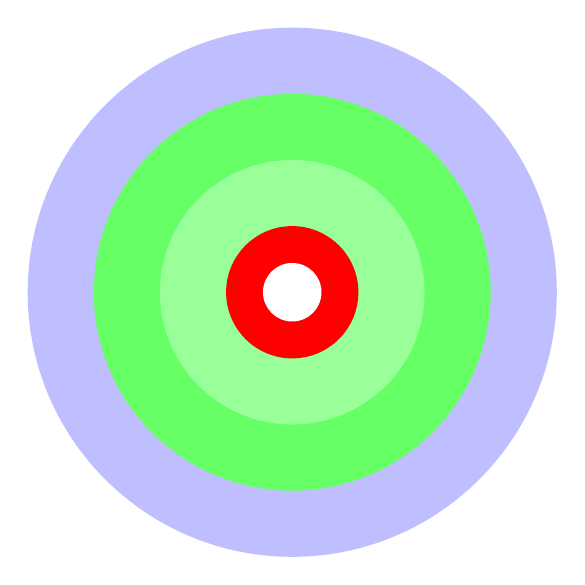
\begin{tikzpicture}[scale=0.42]
			\filldraw[draw=none,fill=blue!25] (0,0) circle (8);
			\filldraw[draw=none,fill=green!60] (0,0) circle (6);
			\filldraw[draw=none,fill=green!40] (0,0) circle (4);
			\filldraw[draw=none,fill=red] (0,0) circle (2);
			\node[fill=black,white,circle,font=\bfseries](nucleus)
			at (0,0) {+};
		\end{tikzpicture}
	\end{center}

		\column{0.4\textwidth}
		With more levels added\ldots
		\begin{itemize}
			\item overlap is greater.
			\item shielding is less effective.
		\end{itemize}
	\end{columns}
\end{frame}

\begin{frame}{Effective Nuclear Charge Practice}
	What is the $Z_\text{eff}$ for the valence electrons in\ldots

	\renewcommand\arraystretch{2}
	\begin{tabular} {*{3}{l}}
		\ch{Rb} & & \\
		\ch{C}  & & \\
		\ch{Se} & & \\
		\ch{F}  & & \\
	\end{tabular}

	And is each element likely to lose or gain an electron?

	\note{
		\begin{center}
		\renewcommand\arraystretch{2}
		\begin{tabular} {*{3}{l}}
			        & $Z_\text{eff} = Z - S$ \\
			\ch{Rb} & $Z_\text{eff} = 37 - 36 = +1$  & lose \\
			\ch{C}  & $Z_\text{eff} = 6 - 2  = +4$   & -- \\
			\ch{Se} & $Z_\text{eff} = 34 -
			\underbrace{28}_{\mathclap{\parbox{\linewidth}{\footnotesize
			\centering The $3d$ orbital is actually considered a
			\alert{core} shell, so we include the 10 electrons here
			-- they are \alert{not} valence \el!}}} = +6$ & gain \\
			\ch{F}  & $Z_\text{eff} = 9 - 2 = +7$    & gain \\
		\end{tabular}
\end{center}}
\end{frame}

\begin{onyourown}%{0em}
	What is the $Z_\text{eff}$ for the valence electrons in\ldots

	\renewcommand\arraystretch{2}
	\begin{tabular} {*{3}{l}}
		\ch{Si} & & \\
		\ch{Fr}  & & \\
		\ch{I} & & \\
		\ch{As}  & & \\
	\end{tabular}

	And is each element likely to lose or gain an electron?
\end{onyourown}

\begin{frame}{Atomic Radii}
	How does the effective nuclear charge affect other atomic properties?

	\begin{center}
		\includegraphics[scale=0.4,trim={0 0 0 40pt},clip]{atomic-radii.jpg}
	\end{center}
\end{frame}

\begin{frame}{Ionic Radii}
	\centering
	\includegraphics[scale=0.4]{cationic-radii.jpg}
	\qquad
	\includegraphics[scale=0.4]{anionic-radii.jpg}
\end{frame}

\begin{frame}{Comparing Relative Radii}
	Rank the following ions in order of decreasing ionic radii by
	filling in the table below:
	
	\begin{center}
		\ch{Na+} \hspace{2em} \ch{Mg^{2+}} \hspace{2em} \ch{Al^{3+}}
	\end{center}

	\begin{center}
		\begin{tabular} {>{\bfseries}l *{3}{>{\centering\arraybackslash}m{0.5in}}}
			\toprule
			& \bfseries \ch{Na+} & \bfseries \ch{Mg^{2+}} &
			\bfseries \ch{Al^{3+}} \\
			\midrule
			\parbox[c][2em][c]{1in}{\ch{e-} config     } \\
			\parbox[c][2em][c]{1in}{\# protons         } \\
			\parbox[c][2em][c]{1in}{\# electrons       } \\
			\parbox[c][2em][c]{1in}{$\bm{Z_\text{eff}}$} \\
			\bottomrule
		\end{tabular}
	\end{center}

	\note{
		\begin{tabular} {>{\bfseries}l *{3}{c}}
		\toprule & \bfseries \ch{Na+} & \bfseries \ch{Mg^{2+}} &
		\bfseries \ch{Al^{3+}} \\
			\midrule
			\ch{e-} config & \elconf{Ne} & \elconf{Ne} & \elconf{Ne} \\
			\# protons & 11 & 12 & 13 \\
			\# electrons & 10 & 10 & 10 \\
			$\bm{Z_\text{eff}}$ & +1 & +2 & +3 \\
			\bottomrule
		\end{tabular}}
\end{frame}

\begin{onyourown}%{0em}
	Rank the following ions in order of decreasing ionic radii by
	filling in the table below:
	
	\begin{center}
		\ch{K+} \hspace{2em} \ch{Ca^{2+}} \hspace{2em} \ch{Ga^{3+}}
	\end{center}

	\begin{center}
		\begin{tabular} {>{\bfseries}l *{3}{c}}
			\toprule
			& \bfseries \ch{K+} & \bfseries \ch{Ca^{2+}} & \bfseries \ch{Ga^{3+}} \\
			\midrule
			\ch{e-} config \\
			\# protons \\
			\# electrons \\
			$\bm{Z_\text{eff}}$ \\
			\bottomrule
		\end{tabular}
	\end{center}
\end{onyourown}

\begin{frame}{Some notes on forming ions\ldots}
	\begin{itemize}[<+->]
		\item For \alert{main group elements}, electrons are removed in
			the reverse order of filling.

			\begin{center}
				\begin{tabular} {l c l}
					F = \elconf{F} & $\rightarrow$ & \ch{F-} =
					$1s^22s^22p^{\color{red}6}$ \\
					Li = \elconf{Li} & $\rightarrow$ &
					\ch{Li+} = $1s^22s^{\color{red}0}$ or
					\elconf{He} \\
				\end{tabular}
			\end{center}

		\item For \alert{transition elements}, remove the electrons in
			the highest $n$-value orbitals first, even if this does
			not correspond to the reverse order of filling.

			\begin{center}
				\begin{tabular} {l c l}
					V = [Ar]$4s^23d^3$ & $\rightarrow$ &
					\ch{V^{2+}} =
					[Ar]$4s^{\color{red}0}3d^3$ or
					[Ar]$3d^3$
				\end{tabular}
			\end{center}

			This deviation has been confirmed experimentally -- in
			particular, this agrees well with the \alert{magnetic
			properties} of the elements/ions.
	\end{itemize}
\end{frame}

\begin{frame}[t]{The Magnetic Properties of Ions}
	Recall $m_s$ -- What does it mean to have a spin of $\pm\frac{1}{2}$?

	\begin{description}
		\item<+(1)->[Paramagnetic:] The atom or ion is \alert{attracted} to a
			magnetic field.
	\end{description}

	\only<.(1)>{%
		\begin{center}
			\begin{tabular} {*{2}{l} *{2}{c}}
				\ch{Ag} & [\ch{Kr}]$5s^14d^{10}$ &
				\electronup & \electronboth \electronboth
				\electronboth \electronboth \electronboth \\
				& & $5s$ & $4d$
			\end{tabular}
		\end{center}
	}

	\begin{description}
		\item<+(1)->[Diamagnetic:] The atom or ion is \alert{slightly repelled}
			by a magnetic field.
	\end{description}

	\only<.(1)>{%
		\begin{center}
			\begin{tabular} {*{2}{l} *{2}{c}}
				\ch{Zn} & [\ch{Ar}]$4s^23d^{10}$ &
				\electronboth & \electronboth \electronboth
				\electronboth \electronboth \electronboth \\
				& & $4s$ & $3d$ \\
				\ch{Zn^{2+}} & [\ch{Ar}]$4s^03d^{10}$ &
				\electronnone & \electronboth \electronboth
				\electronboth \electronboth \electronboth \\
				& & $4s$ & $3d$
			\end{tabular}
		\end{center}
	}
\end{frame}

\begin{frame}{Identifying Magnetism}
	Write the electron configuration and orbital diagram for each ion and
	determine whether each is diamagnetic or paramagnetic.

	\renewcommand\arraystretch{2}
	\begin{tabular} {l *{2}{c}}
		\ch{Al^{3+}}  \\
		\ch{Fe^{3+}}  \\
		\ch{Fe^{2+}}  \\
	\end{tabular}

	\note{%
		\renewcommand\arraystretch{2}
	\begin{tabular} {l *{2}{c}}
		\ch{Al^{3+}} & \elconf{Ne} & diamagnetic \\
		\ch{Fe^{3+}} & [Ar]$3d^5$ & paramagnetic \\
		\ch{Fe^{2+}} & [Ar]$3d^6$ & paramagnetic \\
	\end{tabular}}
\end{frame}

\begin{onyourown}%{0em}
	Write the electron configuration and orbital diagram for each ion and
	determine whether each is diamagnetic or paramagnetic.

	\renewcommand\arraystretch{2}
	\begin{tabular} {l *{2}{c}}
		\ch{Ni^{2+}}  \\
		\ch{Ag^{+}}  \\
		\ch{Ca^{2+}}  \\
	\end{tabular}
\end{onyourown}

\begin{frame}{How easy is it to remove an electron?}
	\begin{columns}
		\column{0.5\textwidth}
		\begin{itemize}[<+->]
			\item We have calculated the energies of atomic orbitals
				before:
				\begin{equation*}
					E_n = -R_{\ch{H}} \bigg( \frac{Z^2}{n^2} \bigg)
				\end{equation*}
			\item As we increase in $n$, we noted that the energy of
				the orbital \alert{increased}.
			\item What happens if we keep increasing $n$?
		\end{itemize}
		\column{0.5\textwidth}
		\visible<3->{%
		\begin{center}
			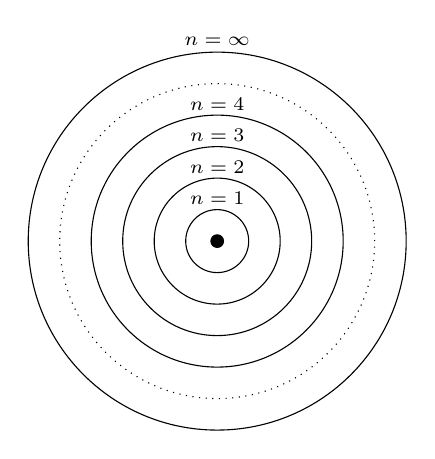
\begin{tikzpicture}[scale=0.4]
				\tikzstyle{every node} = [font=\scriptsize];
				\filldraw[black] (0,0) circle (0.2);
				\foreach \x in {1,2,...,4} {
					\draw[black] (0,0) circle (\x);
					\node[yshift=4pt] at (0,\x) {$n =
					\x$};
					}
				\draw[dotted,black] (0,0) circle (5);
				\draw[black] (0,0) circle (6);
				\node[yshift=4pt] at (0,6) {$n = \infty$};
			\end{tikzpicture}
		\end{center}}
	\end{columns}

	\visible<4->{%
	\begin{block}{Ionization Energy}
		 The energy required to remove an electron from the atom or ion
		 in the gaseous state. Ionization energy is \alert{always}
		 positive.
	\end{block}}
\end{frame}

\vspace{\stretch{-1}}

\begin{frame}[allowframebreaks]{First Ionization Energy}
	The energy required to remove the \alert{first} electron is the
	\alert{first ionization energy}.
	\begin{reaction*}
		Na\gas{} + \text{energy} -> Na^{+}\gas{} + 1 \el
	\end{reaction*}
		
	\begin{itemize}
		\item Decreases going down a group as the distance between the
			nucleus and valence electrons increases.
		\item Increases going across a period from left to right due to
			greater effective nuclear charge.
	\end{itemize}

	\framebreak

	\begin{center}
		\includegraphics[scale=0.4,trim={0 0 0
		40pt},clip]{first-ionization.jpg}
	\end{center}
\end{frame}

\begin{frame}[allowframebreaks]{Second (and Successive) Ionization Energy}
	\begin{columns}
		\column{0.4\textwidth}
		The energy required to remove an electron from an \alert{ion} is
		generally higher than the first ionization energy.
		
		\begin{reactions*}
			&Na^{+}\gas{} + \text{energy} \\
			&\qquad -> Na^{2+}\gas{} + 1 \el
		\end{reactions*}
		\column{0.6\textwidth}
		\begin{center}
			\includegraphics[scale=0.3]{successive-ionization.jpg}
		\end{center}
	\end{columns}

	\framebreak%

	\begin{center}
		\includegraphics[scale=0.42]{ionization-energies.jpg}
	\end{center}
\end{frame}

\vspace{\stretch{-1}}

\begin{frame}{What about gaining electrons?}
	\begin{block}{Electron Affinity}
		The energy change associated with gaining an electron in the
		gaseous state. \alert{Usually negative} because energy is
		released as electrons are gained.
	\end{block}
	\begin{reaction*}
		Cl\gas{} + 1 \el{} -> Cl^{-}\gas{} + \text{energy}
	\end{reaction*}
	\begin{columns}
		\column{0.5\textwidth}
		\begin{itemize}
			\item No significant trend down a column.
			\item Generally becomes more negative across a row.
		\end{itemize}
		\column{0.5\textwidth}
		\begin{center}
			\includegraphics[scale=0.18]{electron-affinities.jpg}
		\end{center}
	\end{columns}
\end{frame}

%\begin{frame}{Trends in Metallic Character}
%	\begin{center}
%		\includegraphics[scale=0.42,trim={0 0 0
%		40pt},clip]{metallic-character.jpg}
%	\end{center}
%\end{frame}

\mode<presentation>{%
	\begin{frame}{Summary of Chapter 3 Periodic Properties}
	\begin{center}
		\includegraphics[scale=0.42]{summary.jpg}
	\end{center}

	\pause

	\begin{block}{Electronegativity (Section 5.2)}
		The ability of an atom to attract electrons to itself in a
		chemical bond. %Results in polar covalent and ionic bonds.
	\end{block}
\end{frame}}

\begin{frame}{Trends in Electronegativity}
	\begin{center}
		\includegraphics[width=\linewidth,trim={0 0 0
		30pt},clip]{05_03_Figure.jpg}
	\end{center}
\end{frame}

\begin{frame}[t]{Electronegativity Example}
	Arrange the following elements in order of \emph{decreasing}
	electronegativity:

	\begin{center}
		\ch{Na} \qquad \ch{Al} \qquad{Mg}
	\end{center}

	\mode<article>{\vspace*{5em}}

	\note{$\ch{Al} > \ch{Mg} > \ch{Na}$}
\end{frame}

\begin{onyourown}%{5em}
	Arrange the following elements in order of \emph{increasing}
	electronegativity:
	
	\begin{center}
		\ch{C} \qquad \ch{Al} \qquad \ch{Si}
	\end{center}
\end{onyourown}

\end{document}
